\chapter{The Mathilda Notebook}
\label{ch:notebook}

Every chapter so far has used Mathilda through its terminal REPL. You type a
line, press Return, and read the answer as text. That is the fastest way to
test an idea, and it is how every transcript in this book was produced. It is
a poor way to keep a record of work. A terminal session cannot hold a heading
or a paragraph of explanation, it prints \(\frac{1}{6}\pi^2\) as
\mcode{1/6 Pi\textasciicircum{}2}, and a plot or an image has nowhere to go.

The \emph{Mathilda Notebook} is the graphical front end that fills that gap.
It is a desktop application in which a document is a list of cells. Some cells
hold Mathilda input and show the result underneath, typeset as mathematics or
drawn as a plot, an image, or a rotatable volume. Other cells hold headings
and prose, with inline \TeX{} for formulas. Several notebooks sit side by side
on an infinite canvas, and any of them can fill the window. The same kernel
that runs in the terminal does all the computing; the notebook only sends it
text and draws what comes back.\index{notebook}\index{front end|see{notebook}}

This chapter covers the notebook from both ends. The first half is a user's
guide: how the pieces fit together, what each kind of output looks like, how
to edit and navigate with the keyboard, what the menus and the toolbar do, and
how to save your work. The second half looks underneath. It shows the exact
messages that pass between the notebook and the kernel, explains how a
three-dimensional volume becomes six textures and then a turning block, and
lists the limitations of the current build honestly. A section of short
featured workflows near the end shows the notebook doing complete small jobs.
Every behaviour described here was checked against the front-end source in
\texttt{frontend/}, and every screenshot in the chapter is the real front end
drawing real kernel output (the method is explained in
\S\ref{sec:nb-screenshots}).

\begin{figure}[htbp]
  \centering
  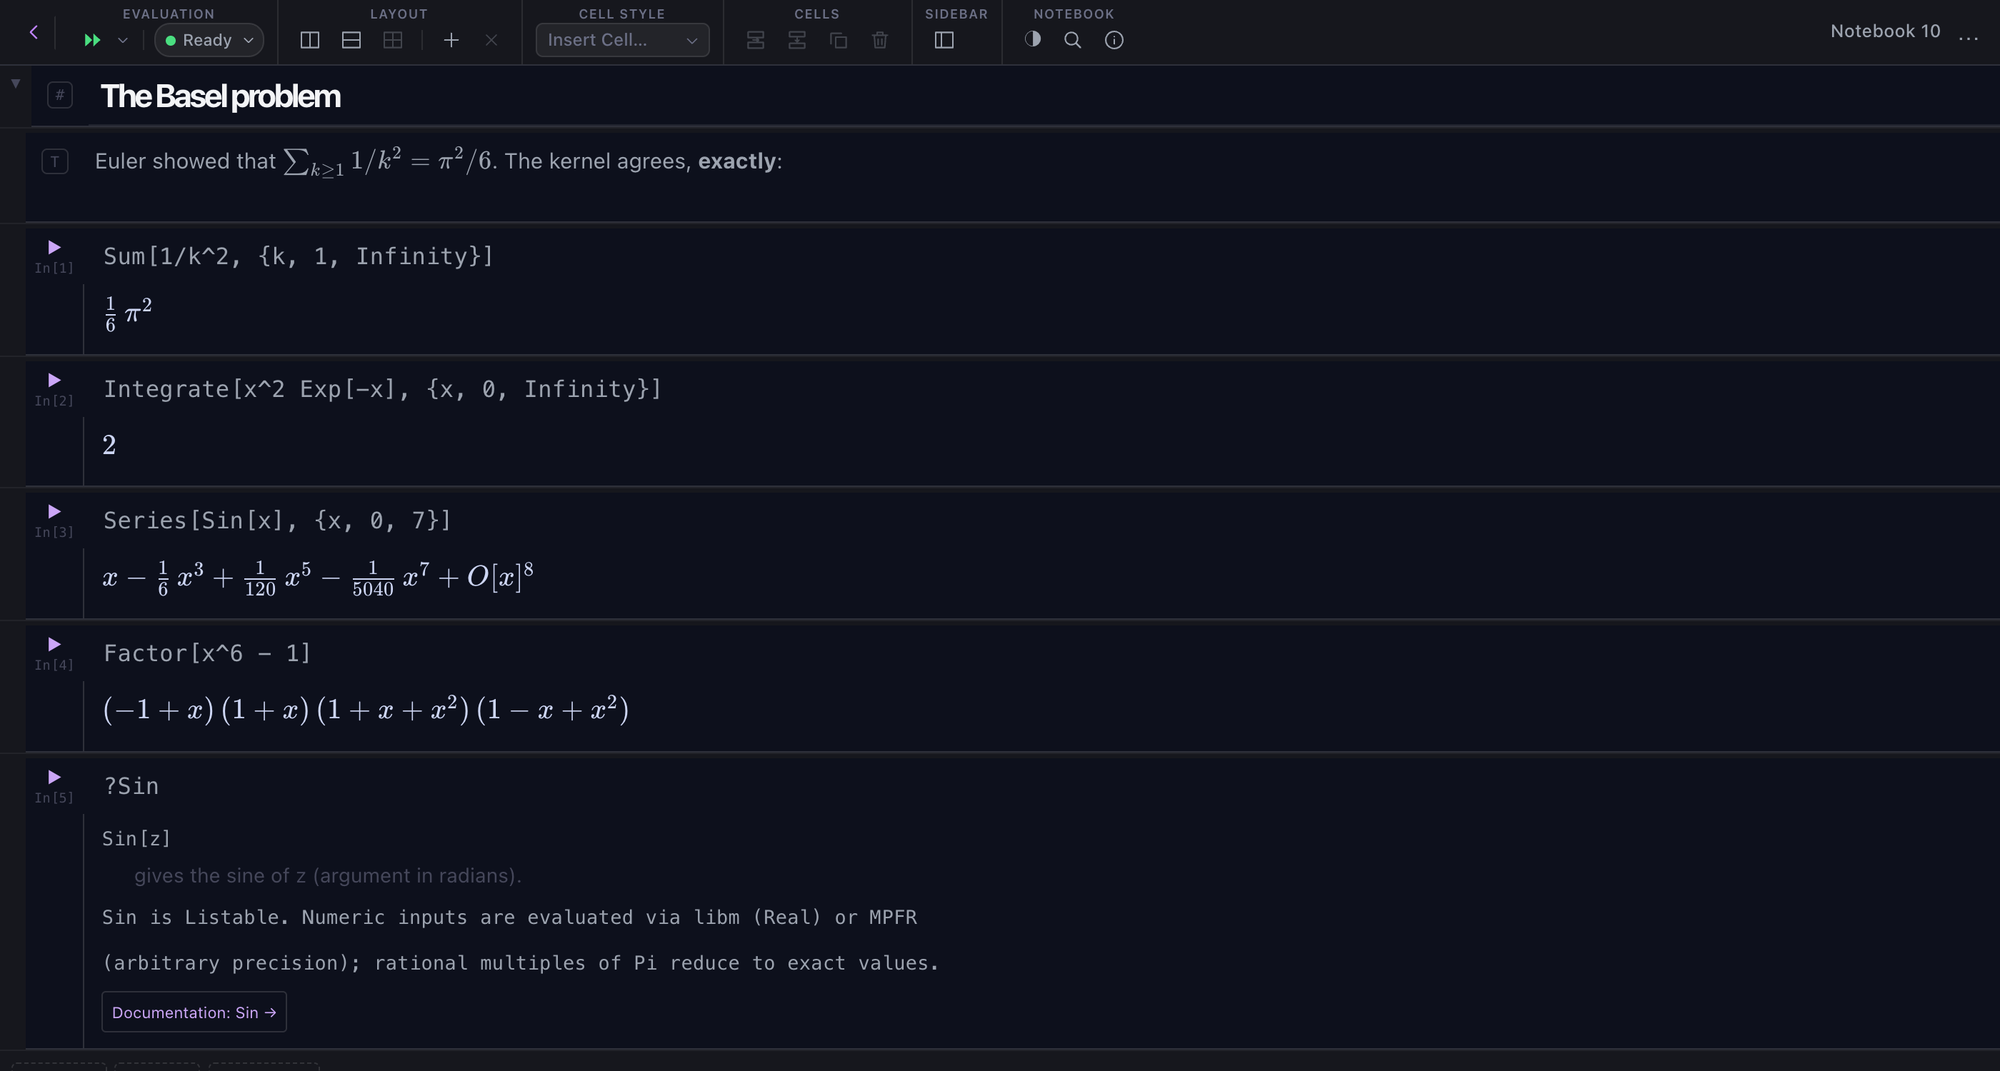
\includegraphics[width=\linewidth]{figures/notebook/report-dark.png}
  \caption{A notebook in focused mode, in the default dark theme. A section
  heading, a text cell with inline \TeX{}, and five evaluated input cells.
  The grouped toolbar runs across the top and the status bar along the
  bottom.}
  \label{fig:nb-report-dark}
\end{figure}

\section{What the notebook is}
\label{sec:nb-overview}

The notebook is a desktop program built with Tauri~2, a framework that pairs
a small native shell written in Rust with a web view that draws the
interface.\index{notebook!Tauri} The interface is written in Svelte and
TypeScript. Input cells are CodeMirror~6 editors, typeset output is rendered
by KaTeX, and plots are drawn by Plotly. The Mathilda kernel is the same C
binary you built in Chapter~\ref{ch:building}. On the desktop the notebook
starts it as a child process and talks to it over its standard input and
output.

The window has two modes.\index{notebook!canvas}\index{notebook!focused mode}
When the program opens you see the \emph{canvas}, a pannable, zoomable plane
holding several notebook cards (Figure~\ref{fig:nb-canvas}). Each card is a
complete notebook with a title bar, and you can drag it, resize it from its
right edge, bottom edge or corner, collapse it, rename it with a
double-click, and run all of its cells from a button in its title bar. A
minimap in the lower left shows every card, and clicking a card there jumps to
it. When you open a card with its full-screen button, the window switches to
\emph{focused mode}. The card fills the window, its title bar is replaced by
the grouped toolbar shown in Figure~\ref{fig:nb-report-dark}, and an optional
status bar appears along the bottom. Up to four notebooks can share the window
in focused mode, side by side, stacked, or in a two-by-two grid.

\begin{figure}[htbp]
  \centering
  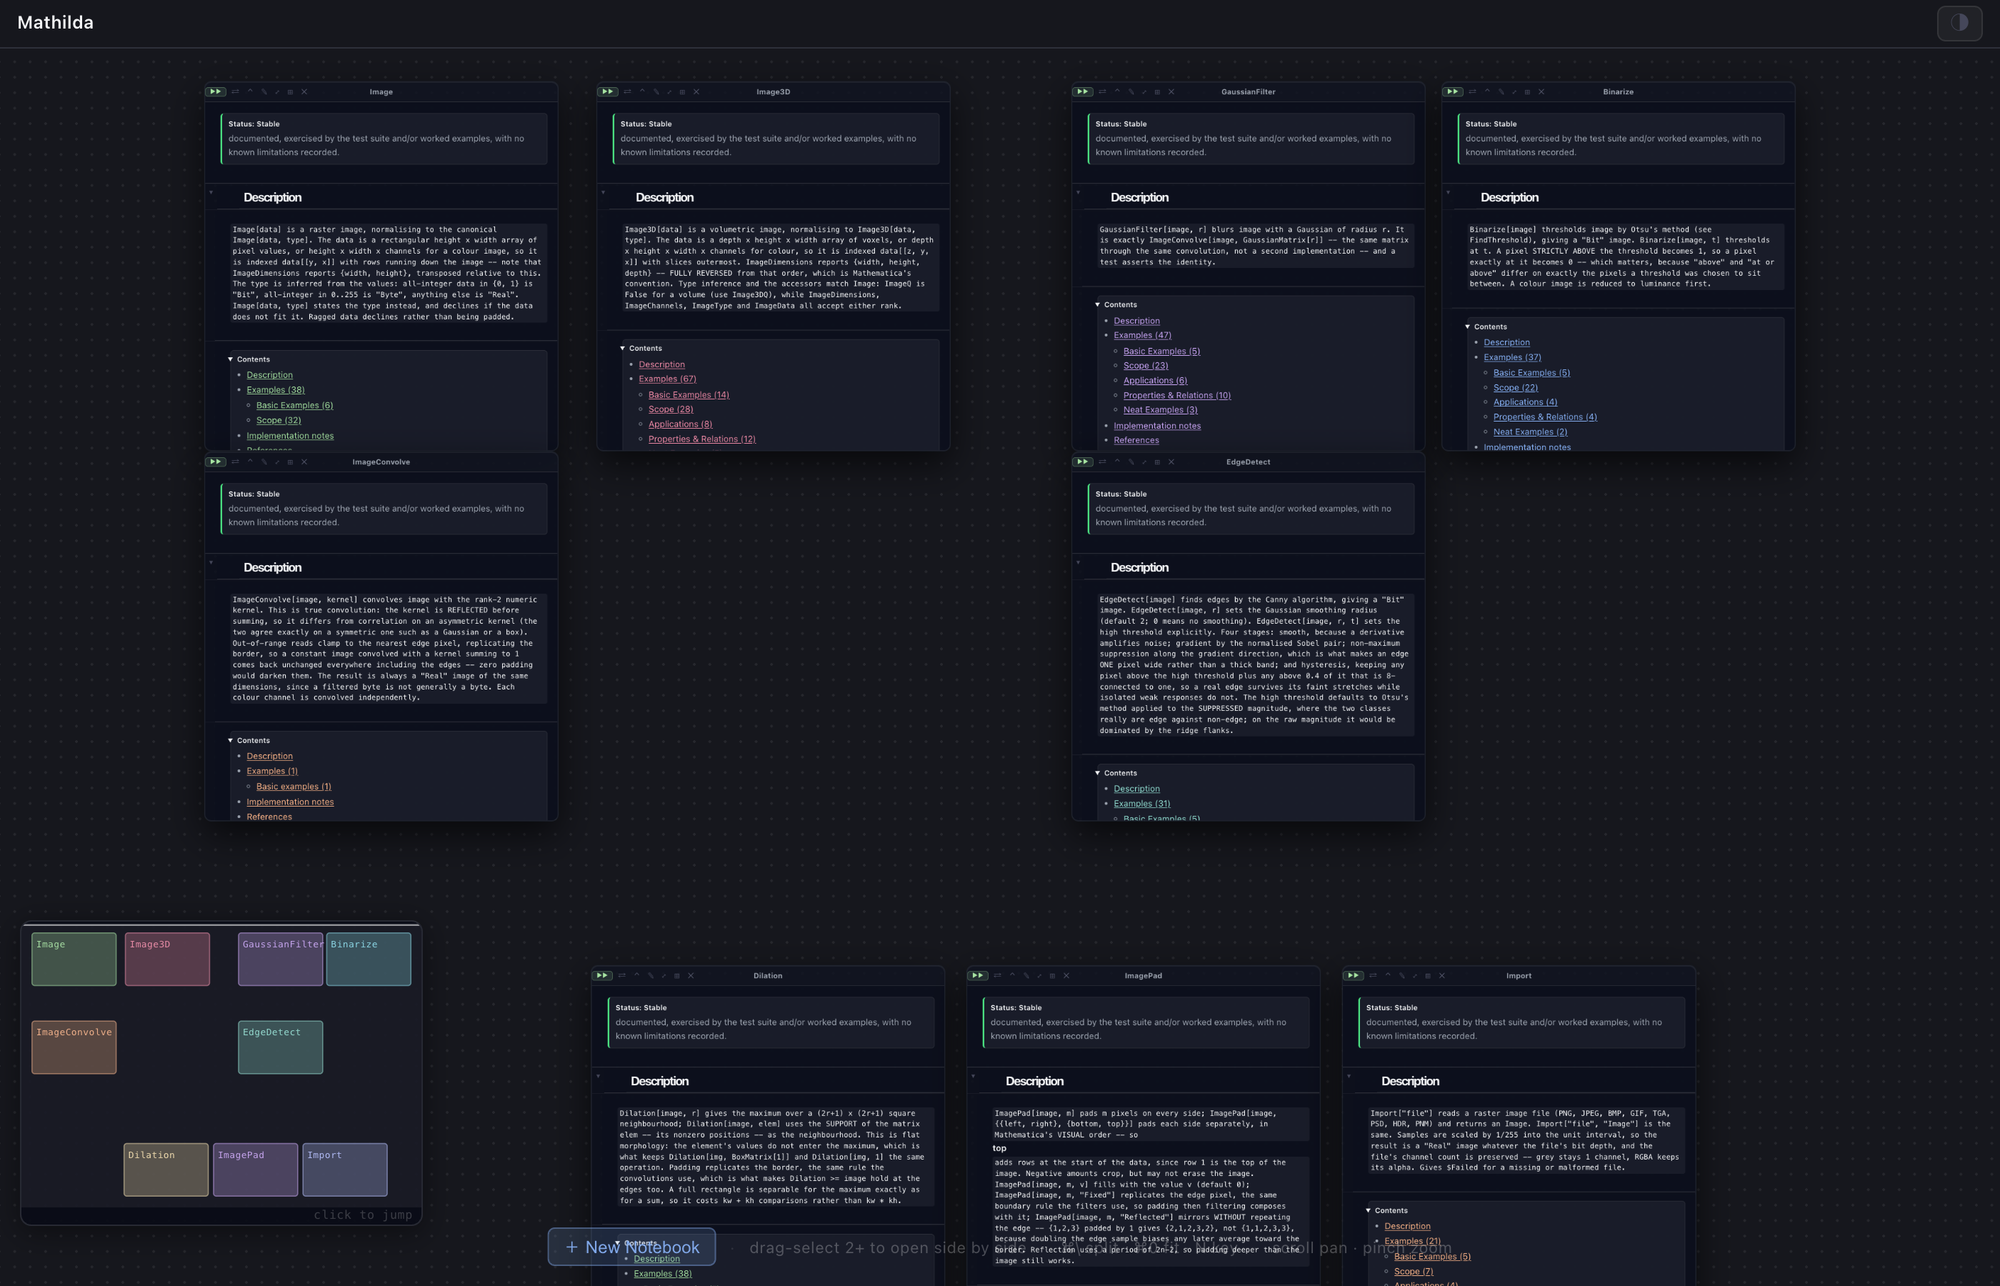
\includegraphics[width=\linewidth]{figures/notebook/canvas.png}
  \caption{The canvas as the notebook opens it, fitted to the window with
  \texttt{Cmd+0}. The nine starter cards are the reference pages of the image
  subsystem, each a live notebook. The minimap is in the lower left.}
  \label{fig:nb-canvas}
\end{figure}

The canvas opens on nine reference pages: \B{Image}, \B{Image3D},
\B{ImageConvolve}, \B{GaussianFilter}, \B{EdgeDetect}, \B{Binarize},
\B{Dilation}, \B{ImagePad}, and \B{Import}. These are the same generated pages
that the Mathilda website publishes, converted into notebooks so that every
example on them is an input cell you can edit and run again
(\S\ref{sec:nb-docs}). The source keeps an older starter set as well, a tour
of calculus, plots, number theory, linear algebra and associations, and a
comment in \texttt{canvas.ts} notes that one line in \texttt{Canvas.svelte}
switches between the two.

\paragraph{Platforms.} The desktop build is the primary target, and the code
contains several macOS-specific decisions: the menus live in the macOS menu
bar, the build script ad-hoc signs the kernel binary for Apple
Silicon, and the keyboard shortcuts are written for the Command key.
\index{notebook!platforms} The Tauri configuration asks for bundles on every
platform Tauri supports (a \texttt{.app} on macOS, \texttt{.deb} on Linux,
\texttt{.msi} on Windows), and \texttt{Ctrl} is accepted wherever the code
checks for \texttt{Cmd}. The Linux and Windows bundles are configured but are
not covered by any test in the repository, so treat them as untested. There
are also iOS and Android builds, which run the kernel inside the app instead
of as a separate process. They are described in \S\ref{sec:nb-mobile} and are
more limited than the desktop build.

\section{Architecture}
\label{sec:nb-architecture}

The notebook has three layers, and it helps to keep them apart when something
goes wrong (Figure~\ref{fig:nb-arch}).\index{notebook!architecture}

\begin{figure}[htbp]
\centering
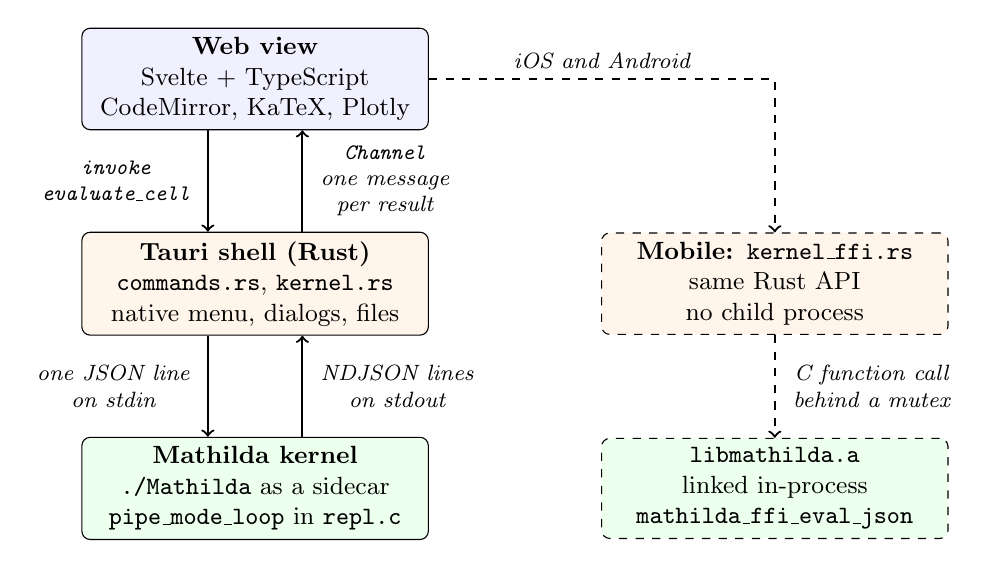
\begin{tikzpicture}[
  box/.style={draw, rounded corners=3pt, align=center, minimum width=4.4cm,
              minimum height=1.25cm, font=\small},
  lab/.style={font=\footnotesize\itshape, align=center}]
  % desktop column
  \node[box, fill=blue!6] (ui) at (0,0)
     {\textbf{Web view}\\Svelte + TypeScript\\CodeMirror, KaTeX, Plotly};
  \node[box, fill=orange!8] (rust) at (0,-2.6)
     {\textbf{Tauri shell (Rust)}\\\texttt{commands.rs}, \texttt{kernel.rs}\\native menu, dialogs, files};
  \node[box, fill=green!7] (kern) at (0,-5.2)
     {\textbf{Mathilda kernel}\\\texttt{./Mathilda} as a sidecar\\\texttt{pipe\_mode\_loop} in \texttt{repl.c}};
  \draw[->, thick] ([xshift=-6mm]ui.south) -- node[lab, left=1mm] {\texttt{invoke}\\\texttt{evaluate\_cell}} ([xshift=-6mm]rust.north);
  \draw[<-, thick] ([xshift=6mm]ui.south) -- node[lab, right=1mm] {\texttt{Channel}\\one message\\per result} ([xshift=6mm]rust.north);
  \draw[->, thick] ([xshift=-6mm]rust.south) -- node[lab, left=1mm] {one JSON line\\on stdin} ([xshift=-6mm]kern.north);
  \draw[<-, thick] ([xshift=6mm]rust.south) -- node[lab, right=1mm] {NDJSON lines\\on stdout} ([xshift=6mm]kern.north);
  % mobile column
  \node[box, fill=orange!8, dashed] (ffi) at (6.6,-2.6)
     {\textbf{Mobile: \texttt{kernel\_ffi.rs}}\\same Rust API\\no child process};
  \node[box, fill=green!7, dashed] (lib) at (6.6,-5.2)
     {\textbf{\texttt{libmathilda.a}}\\linked in-process\\\texttt{mathilda\_ffi\_eval\_json}};
  \draw[->, thick, dashed] (ffi.south) -- node[lab, right=1mm] {C function call\\behind a mutex} (lib.north);
  \draw[->, thick, dashed] (ui.east) -| node[lab, above, pos=0.25] {iOS and Android} (ffi.north);
\end{tikzpicture}
\caption{The three layers of the notebook. On the desktop the Rust shell
spawns the kernel binary and relays JSON lines. On iOS and Android the kernel
is a static library called directly from Rust, because those systems do not
allow an app to start a child process.}
\label{fig:nb-arch}
\end{figure}

\paragraph{The web view} draws everything you see and holds the notebook in
memory. A notebook is a Svelte store, an observable value, holding a list of
rows (\S\ref{sec:nb-cells}). The web view never touches the kernel directly.
To evaluate a cell it calls the Tauri command \mcode{evaluate\_cell} with the
cell's source text and a \emph{channel}, a callback that the Rust side can
call many times. Each message the kernel produces for that cell arrives
through the channel and is appended to the cell's output.

\paragraph{The Rust shell} is small. \texttt{lib.rs} builds the native menu
bar and registers nine commands: evaluate, restart, interrupt, ping, save and
load a notebook, save and load a library, and set the window title.
\texttt{kernel.rs} owns the kernel process. It holds the child process, its
output stream, and a request counter behind one asynchronous mutex, so only
one evaluation runs at a time, whichever notebook asked for it.

\paragraph{The kernel} is the unmodified \texttt{Mathilda} binary. When its
standard input is not a terminal and no script file was named, it enters the
pipe mode that \S\ref{sec:scripts} mentioned and speaks a line-oriented JSON
protocol instead of showing a prompt. The next section describes that
protocol in full.%
\calloutnote{Under the hood}{Tauri calls the bundled binary a
\emph{sidecar}. The build script \texttt{build-sidecar.sh} compiles Mathilda
with \texttt{make USE\_ECM=0} and copies it into
\texttt{src-tauri/binaries/} with the Rust target triple appended to the file
name, which is the naming Tauri requires. The script also replaces any copy
that an earlier \texttt{cargo} build placed in \texttt{target/debug} or
\texttt{target/release}, because those copies are what a running development
build executes. It replaces them with a move, never by writing over the file:
on macOS, overwriting a binary that a running process has mapped invalidates
its code signature, and the replacement is then killed when it starts.}

\paragraph{One kernel for every notebook.} There is exactly one kernel
process, shared by every card on the canvas.\index{notebook!shared kernel}
If you define \mcode{f[x\_] := x\textasciicircum{}2} in one notebook, \mcode{f[3]} returns
\mcode{9} in every other notebook. Evaluating a whole notebook does not
restart the kernel first, so a notebook that relies on a definition made in a
different notebook will appear to work until the kernel restarts. When two
panes evaluate at once, the second waits for the mutex, and the status bar's
timing for that cell includes the wait.

\paragraph{Starting up.} When the app starts, Rust spawns the sidecar in the
background and sends \mcode{\{"type":"ping"\}}. The kernel answers
\mcode{\{"type":"pong"\}} once it has loaded its builtins and
\texttt{init.m}. Rust waits up to ten seconds for that answer. The web view,
meanwhile, shows the kernel as \emph{Starting}, waits 1.2 seconds, and sends
its own ping. If the ping fails, the kernel is shown as \emph{Not running} and
a red banner offers a Restart button.

\section{The kernel protocol}
\label{sec:nb-protocol}
\index{notebook!NDJSON protocol}\index{NDJSON protocol}

The protocol is \emph{NDJSON}, newline-delimited JSON. Each request is one
JSON object on one line of the kernel's standard input. Each response is one
JSON object on one line of its standard output. The kernel sets its output to
unbuffered in pipe mode so that every line reaches the pipe as soon as it is
written. Because the protocol is plain text, you can drive it from a shell
with no notebook at all, and seeing it this way is the quickest route to
understanding what the notebook receives:

\begin{shell}
$ printf '%s\n' '{"type":"ping"}' \
    '{"id":1,"expr":"Integrate[x^2, {x, 0, 1}]"}' \
    '{"id":2,"expr":"Factor[x^4 - 1]"}' \
    '{"id":3,"expr":"f[x"}' | ./Mathilda 2>/dev/null
{"type":"pong"}
{"id":1,"type":"expr","payload":"1/3","latex":"\\frac{1}{3}"}
{"id":1,"type":"done","memory":18612224}
{"id":2,"type":"expr","payload":"(-1 + x) (1 + x) (1 + x^2)","latex":"(-1+x)\\,(1+x)\\,(1+x^{2})"}
{"id":2,"type":"done","memory":19595264}
{"id":3,"type":"error","message":"Parse error: f[x"}
{"id":3,"type":"done","memory":19595264}
\end{shell}

These lines were captured from the binary the book was built with; only the
shell prompt was added. A request carries an integer \mcode{id} and the input
text as \mcode{expr}. Every response to that request repeats the \mcode{id},
and the last one has \mcode{"type":"done"}. The notebook uses the \mcode{id}
to ignore stray lines and the \mcode{done} line to know that the cell is
finished. The \mcode{memory} field on \mcode{done} is the kernel's resident
memory in bytes, which the status bar shows. A parse error echoes the exact
text that was received, so an invisible character or an unbalanced bracket in
the input can be found.

\begin{sloppypar}
Two requests have no \mcode{id}. \mcode{\{"type":"ping"\}} is answered with
\mcode{\{"type":"pong"\}}, and \mcode{\{"type":"quit"\}} makes the kernel
leave its loop and exit. The Rust shell sends \mcode{quit} before it kills the
process during a restart.
\end{sloppypar}

\subsection{How the kernel classifies a result}

After evaluating the input, the kernel decides what kind of message to send.
The decision is made on the evaluated expression, in this order:

\begin{enumerate}
\item If the input was a help query, \mcode{?name} or
  \mcode{Information[name]}, possibly as the last element of a
  \B{CompoundExpression}, the result is documentation. A list of names (from
  \mcode{?Prime*}) is sent as a \mcode{names} message. A docstring is sent as
  a \mcode{usage} message, together with the symbol it describes, so that the
  notebook can link to that symbol's page.
\item If the result has head \mcode{Image} or \mcode{Image3D} and can be read
  as a raster, it is sent as an \mcode{image} message carrying the pixels.
\item If the result has head \mcode{Graphics} or \mcode{Graphics3D}, it is
  converted to a Plotly figure and sent as a \mcode{plot} message.
\item Anything else is printed as text, the same text the REPL shows, and is
  also converted to \LaTeX{}. Both go in one \mcode{expr} message.
\end{enumerate}

\begin{shell}
$ printf '%s\n' '{"id":5,"expr":"?Sin"}' '{"id":6,"expr":"?Prime*"}' \
    '{"id":9,"expr":"Image[{{0, 0.5}, {1, 0.25}}]"}' | ./Mathilda 2>/dev/null
{"id":5,"type":"usage","payload":"Sin[z]\n\tgives the sine of z (argument in radians).\nSin is Listable. Numeric inputs are evaluated via libm (Real) or MPFR\n(arbitrary precision); rational multiples of Pi reduce to exact values.","symbol":"Sin"}
{"id":5,"type":"done","memory":19611648}
{"id":6,"type":"names","payload":["Prime","PrimeNu","PrimeOmega","PrimePi","PrimeQ"]}
{"id":6,"type":"done","memory":19611648}
{"id":9,"type":"image","payload":{"w":2,"h":2,"channels":1,"data":"AAAA/4CAgP//////QEBA/w=="}}
{"id":9,"type":"done","memory":19611648}
\end{shell}

Table~\ref{tab:nb-messages} lists every message type the desktop kernel
sends. The \mcode{data} field of an image is base64-encoded RGBA, four bytes
per pixel, row by row. The two-by-two image above decodes to the grey levels
0, 128, 255 and 64, each followed by an opaque alpha byte of 255.

\begin{table}[htbp]
\centering
\small
\begin{tabular}{@{}lll@{}}
\toprule
\textbf{\texttt{type}} & \textbf{Fields} & \textbf{Sent when} \\
\midrule
\texttt{pong}  & (no \texttt{id}) & answer to a ping \\
\texttt{expr}  & \texttt{payload}, \texttt{latex} & an ordinary result \\
\texttt{usage} & \texttt{payload}, \texttt{symbol} & \texttt{?name} gave a docstring \\
\texttt{names} & \texttt{payload} (array) & \texttt{?pattern*} gave a list of names \\
\texttt{image} & \texttt{payload}: \texttt{w}, \texttt{h}, \texttt{channels}, \texttt{data} & the result is an \texttt{Image} \\
       & \quad plus \texttt{depth}, \texttt{slice}, \texttt{faces} & \quad or an \texttt{Image3D} \\
\texttt{plot}  & \texttt{payload}: \texttt{data}, \texttt{layout} & the result is \texttt{Graphics} or \texttt{Graphics3D} \\
\texttt{error} & \texttt{message} & a parse error, or out of memory \\
\texttt{done}  & \texttt{memory} & always last for each request \\
\bottomrule
\end{tabular}
\caption{The messages the desktop kernel writes in pipe mode.}
\label{tab:nb-messages}
\end{table}

A \mcode{plot} payload is an ordinary Plotly figure specification. For
\mcode{Plot[Sin[x], \{x, 0, 1\}]} the kernel sends one trace of
\mcode{"type":"scatter"} with \mcode{"mode":"lines"}, the sample points as
\mcode{x} and \mcode{y} arrays, a line colour and width, and a \mcode{layout}
object with grid, margin and height settings. The notebook hands this to
Plotly almost unchanged (\S\ref{ssec:nb-plots}).

\subsection{What the notebook does to your input}

Before a cell's text is sent, the notebook replaces typographic characters
that a web view or a word processor may have substituted. Curly quotes become
straight quotes, en dashes, em dashes and the minus sign become a hyphen, and
the arrow \(\rightarrow\) becomes \mcode{->}. None of these characters means
anything distinct in Mathilda input, and left alone they would turn
\mcode{->} into a parse error or break a string. The text is then placed in
the \mcode{expr} field with standard JSON escaping.%
\calloutnote{Pitfall}{A cell is sent as one request, and the kernel parses it
as \emph{one} expression. Newlines are whitespace to Mathilda's parser, so a
cell holding \mcode{a = 2}, \mcode{b = 3} and \mcode{a + b} on three lines is
a parse error. Join statements with semicolons, \mcode{a = 2; b = 3; a + b},
which is a \B{CompoundExpression} whose value is the last part. The kernel
also reads each request into a buffer of 10\,240 bytes, so a single cell
longer than about ten kilobytes, after JSON escaping, is cut off.}

\subsection{What does not reach the notebook}
\label{ssec:nb-lost}

Two kinds of kernel output never appear in a cell. The first is anything a
program prints. \B{Print} writes its text straight to standard output, where
it arrives as a line that is not JSON. The Rust shell logs a parse warning for
such a line and drops it. The second is warning messages. Mathilda writes
messages such as \mcode{Power::infy} to standard error, which the shell sends
to its debug log only. So \mcode{1/0} shows \mcode{ComplexInfinity} with no
warning, and a cell that only calls \mcode{Print} shows nothing at all.
\index{notebook!limitations}

The front end is ready for printed output. Its message type list includes a
\mcode{stream} type, and consecutive \mcode{stream} messages are merged into
one block of preformatted text, but the desktop kernel does not yet send that
type. The same list includes an \mcode{html} type, which the notebook uses
internally for recorded pictures on reference pages.%
\calloutnote{Under the hood}{The kernel does not contain a JSON parser. The
functions \texttt{json\_get\_int} and \texttt{json\_get\_string} in
\texttt{repl.c} find the quoted key with \texttt{strstr} and read the value
that follows, undoing the common backslash escapes. Ping and quit are
recognised by searching the whole line for the quoted words
\texttt{"ping"} and \texttt{"quit"}, before the \texttt{expr} field is read.
This is safe only because of JSON escaping: a Mathilda string such as
\mcode{"quit"} inside a cell travels as
\texttt{\textbackslash"quit\textbackslash"}, where a backslash, not a quote,
follows the word, so it never matches. The approach is enough for the
requests the notebook sends, which always have the same shape, but it is not a
general JSON reader.}

\begin{figure}[htbp]
\centering
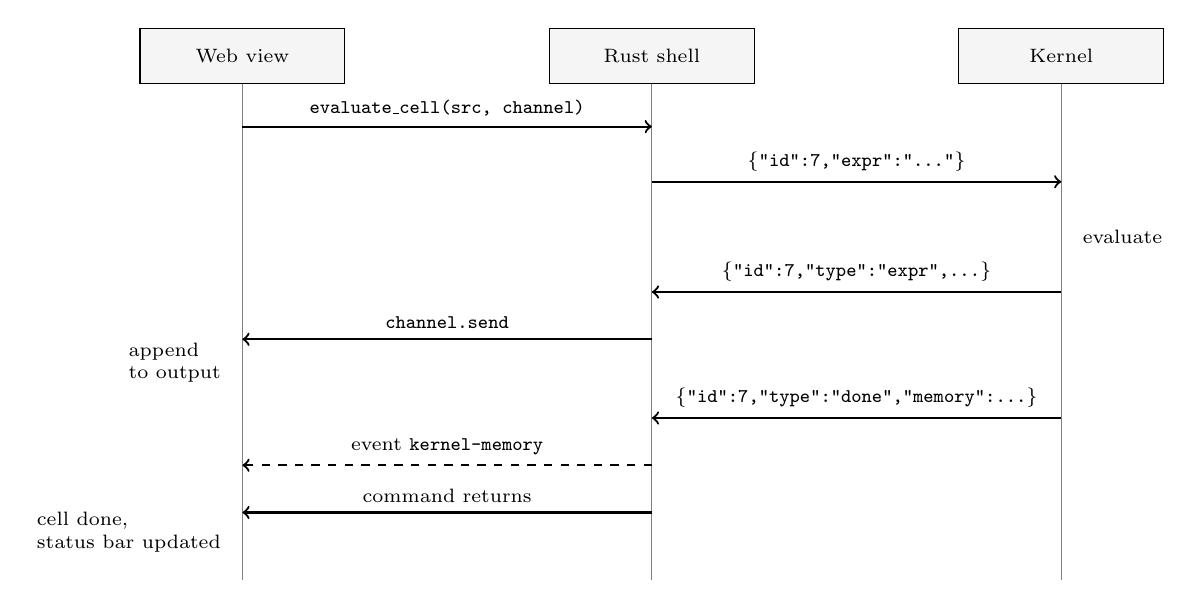
\begin{tikzpicture}[font=\scriptsize,
  lane/.style={draw, fill=gray!8, minimum width=2.6cm, minimum height=0.7cm, align=center},
  msg/.style={->, thick}]
  \node[lane] (w) at (0,0) {Web view};
  \node[lane] (r) at (5.2,0) {Rust shell};
  \node[lane] (k) at (10.4,0) {Kernel};
  \foreach \n in {w,r,k} \draw[gray] (\n.south) -- ++(0,-6.3);
  \draw[msg] (0,-0.9) -- node[above] {\texttt{evaluate\_cell(src, channel)}} (5.2,-0.9);
  \draw[msg] (5.2,-1.6) -- node[above] {\texttt{\{"id":7,"expr":"..."\}}} (10.4,-1.6);
  \node[align=left, anchor=west] at (10.55,-2.3) {evaluate};
  \draw[msg] (10.4,-3.0) -- node[above] {\texttt{\{"id":7,"type":"expr",...\}}} (5.2,-3.0);
  \draw[msg] (5.2,-3.6) -- node[above] {\texttt{channel.send}} (0,-3.6);
  \node[align=left, anchor=east] at (-0.15,-3.9) {append\\to output};
  \draw[msg] (10.4,-4.6) -- node[above] {\texttt{\{"id":7,"type":"done","memory":...\}}} (5.2,-4.6);
  \draw[msg, dashed] (5.2,-5.2) -- node[above] {event \texttt{kernel-memory}} (0,-5.2);
  \draw[msg] (5.2,-5.8) -- node[above] {command returns} (0,-5.8);
  \node[align=left, anchor=east] at (-0.15,-6.05) {cell done,\\status bar updated};
\end{tikzpicture}
\caption{One evaluation. The request counter in Rust supplies the
\texttt{id}. Result messages travel through the cell's channel; the memory
figure on \texttt{done} travels as a separate event, because it is not part
of the cell's output.}
\label{fig:nb-sequence}
\end{figure}


\section{Notebooks, rows and cells}
\label{sec:nb-cells}
\index{notebook!cells}

A notebook is a list of \emph{rows}, and each row holds one or more
\emph{cells} placed side by side. Most rows hold one cell. The row structure
exists so that a cell can be inserted to the left or right of another, and
the store's operations are written in terms of rows. Each cell has an id, a
type, its source text, a status (idle, running, done or error), a list of
output items, and, once it has run, an execution number shown as
\mcode{In[n]} in the gutter.

There are five cell types. Four of them you create and edit yourself.

\begin{description}
\item[Code] An input cell. The source is Mathilda text in a CodeMirror
  editor, and the results appear under it. Only code cells are ever sent to
  the kernel, and a code cell whose source is empty or blank is skipped.
\item[Text] Prose, written in Markdown with inline \TeX{} between dollar
  signs (\S\ref{sec:nb-text}). The cell shows the rendered text until you
  click into it, and the raw source while you edit.
\item[Section] A top-level heading. Clicking the fold marker in the margin
  hides every row up to the next section.
\item[Subsection] A second-level heading, folding the rows up to the next
  heading of either level.
\item[Reference] Read-only generated documentation. Reference pages use this
  type for their prose, and you cannot retype such a cell or edit its text.
\end{description}

Changing a cell's type keeps its output. Only code cells draw an output area,
so a result is hidden while the cell is a text cell and comes back if you
change it to code again. The execution counter that produces the
\mcode{In[n]} labels is a single counter shared by every notebook in the
window, so numbers keep rising as you move between notebooks. Evaluating a
whole notebook resets it to zero first, and running one cell or a range
does not. The labels can be hidden in the properties panel
(\S\ref{sec:nb-kernel}).

Folding is nested correctly. Collapsing a subsection hides only the rows
under it, up to the next heading, and collapsing a section hides its
subsections and everything in them. Content rows are indented one step under
a section and two under a subsection, so the structure is visible without
folding anything. Every notebook with headings also gets a single button,
in the card title bar and in the toolbar's overflow menu, that collapses
every heading while any is open and expands them all once all are closed.

\section{Text cells: Markdown and \TeX{}}
\label{sec:nb-text}
\index{notebook!text cells}\index{notebook!Markdown}

A text cell is rendered as Markdown by the \texttt{marked} library, with
GitHub-flavoured extensions and one setting that matters in practice: a
single Return is a line break. You type a text cell like prose, and needing
two trailing spaces to end a line would feel like the cell was ignoring the
Return key. An empty text cell opens in edit mode, since an empty rendered
cell has no height to click on.

Mathematics goes between dollar signs, \mcode{\$\ldots\$} for inline and
\mcode{\$\$\ldots\$\$} for display, and is rendered by KaTeX. The text cell in
Figure~\ref{fig:nb-report-dark} was typed as

\begin{shell}
Euler showed that $\sum_{k\ge 1} 1/k^2 = \pi^2/6$. The kernel agrees, **exactly**:
\end{shell}

The math is pulled out of the text \emph{before} Markdown runs and put back
afterwards. The order matters. Markdown treats underscores and asterisks as
emphasis, so \mcode{\$a\_1 * b\_2\$} handed to Markdown first would lose
\mcode{\_1 * b\_2} to italics, and nothing afterwards could recover it. The
scan that extracts math is hand-written because the cases that must not be
math depend on context. A dollar sign inside a code span or a fenced block is
a literal dollar, and \mcode{\textbackslash\$} is a literal dollar anywhere.%
\calloutnote{Pitfall}{Two rules keep prose about money from turning into
formulas, the same two that pandoc and markdown-it use. An opening dollar
must be followed by a non-space character, and a closing dollar must be
preceded by one. So \emph{it cost \$5 and \$6} stays prose, while
\mcode{\$x + 1\$} is math. An unclosed dollar is left exactly as typed. If a
formula refuses to render, check for a space just inside a delimiter.}

When a text cell is active, the toolbar shows a \emph{Text} group with five
buttons: bold, italic, inline code, link, and inline math. Each wraps the
selection in the corresponding markers (\mcode{**}, \mcode{*}, a backtick,
\mcode{[text](url)}, or \mcode{\$}). The edit goes through the browser's
native undo stack, so \texttt{Cmd+Z} undoes it. The group does not appear for
section and subsection cells, because headings are not rendered as Markdown
and the markers would show as literal characters. There is no bullet-list
button, and clicking into rendered prose places the caret where focus puts
it, not at the clicked character. Both would need a mapping from a position
in the rendered text back to a position in the source, and the source
comments explain that a wrong mapping is worse than none.

Rendered prose reaches the page as raw HTML, and the code does not sanitise
it. The comment in \texttt{prose.ts} gives the reasoning: a notebook's code
cells already run arbitrary Mathilda, so a notebook from someone you do not
trust is unsafe to run whether or not its prose contains HTML.

\section{How results are drawn}
\label{sec:nb-outputs}
\index{notebook!output rendering}

Each message from the kernel becomes one output item under the cell, and
each kind of item has its own renderer. Figure~\ref{fig:nb-report} shows the
common cases in the light theme.

\begin{figure}[htbp]
  \centering
  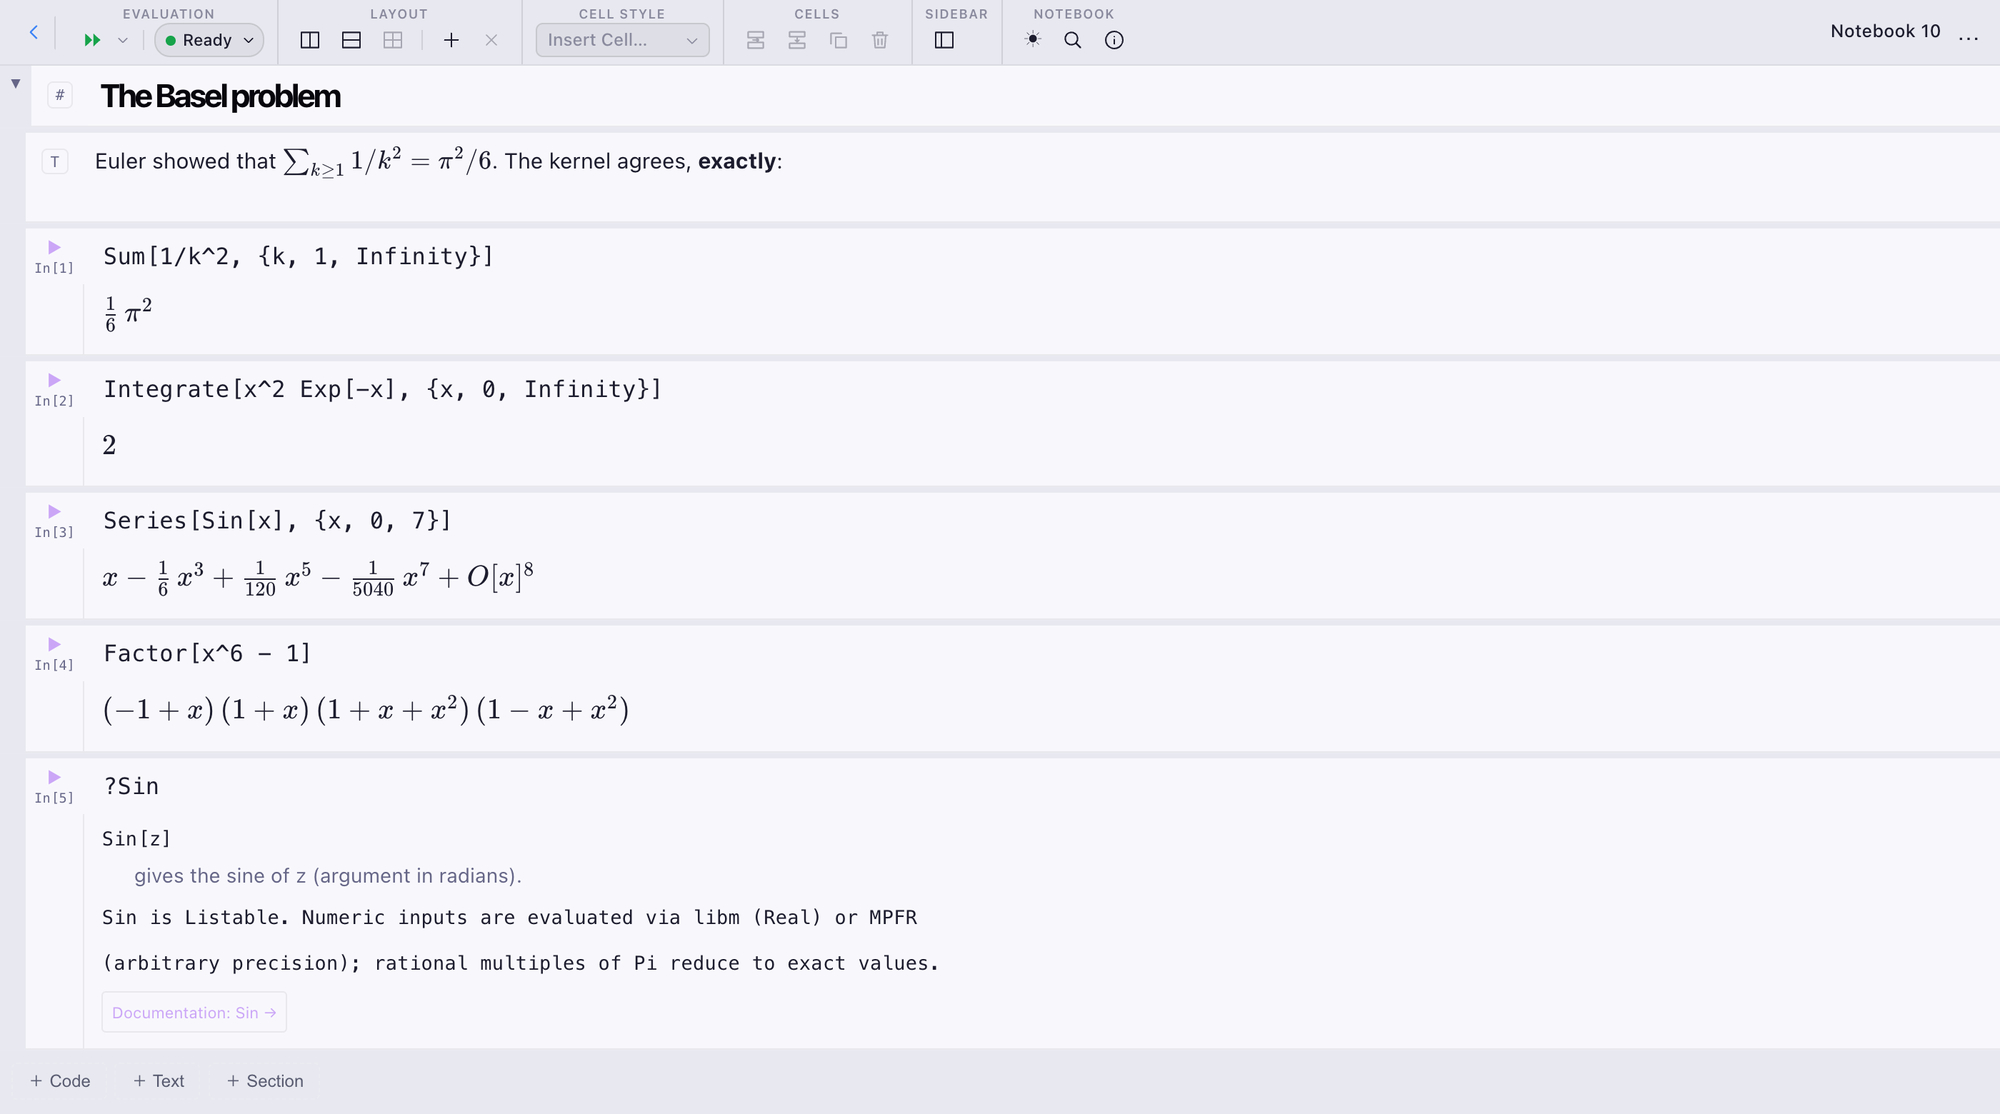
\includegraphics[width=\linewidth]{figures/notebook/report.png}
  \caption{Typeset results and a usage message in the light theme. A sum, a
  definite integral, a series with its order term, a factorisation, and the
  help text for \texttt{Sin} with a button that opens its reference page.}
  \label{fig:nb-report}
\end{figure}

\subsection{Expressions}

An \mcode{expr} message carries both the plain text and the \LaTeX{} form.
The notebook prefers the \LaTeX{} and renders it with KaTeX, so
\mcode{Sum[1/k\textasciicircum{}2, \{k, 1, Infinity\}]} is shown as a fraction times
\(\pi^2\), and a series shows its \(O[x]^8\) term with a real superscript. The
\LaTeX{} comes from the kernel's own \emph{StandardForm} serialiser, the
routine \texttt{expr\_to\_latex}, so the notebook does no conversion of its
own.

Long results are handled differently. KaTeX cannot break a formula across
lines, so a result with more than four commas, or more than 200 characters
of text, is shown as wrapping monospace text instead. The rule catches long
lists, which gain nothing from typesetting. The list of primes in
Figure~\ref{fig:nb-side} is an example. If KaTeX fails on a formula it shows
its own error marker in place, and the rest of the cell still renders.

Any text output taller than 180 pixels is clipped with a fade at the bottom
and a \emph{show all} link. The notebook measures the height again whenever
the output resizes, so widening a card can remove the clip and narrowing it
can add one.

\subsection{Help and names}

A \mcode{usage} message is documentation, and it is never typeset. The
docstrings are written for an 80-column terminal, with a signature flush left
and a description indented under it. The notebook parses that layout back
into signature lines, set in monospace, and description paragraphs, set as
ordinary text, then adds a \emph{Documentation} button when the message names
its symbol. The button opens that symbol's reference page beside the notebook
(\S\ref{sec:nb-docs}).

A \mcode{names} message becomes a grid of names. Each name is a button that
opens that symbol's reference page, so \mcode{?Image*} works as a browser for
the image subsystem. The toolbar's \emph{Browse all symbols} command is simply
a new notebook that evaluates \mcode{?*}.

\begin{figure}[htbp]
  \centering
  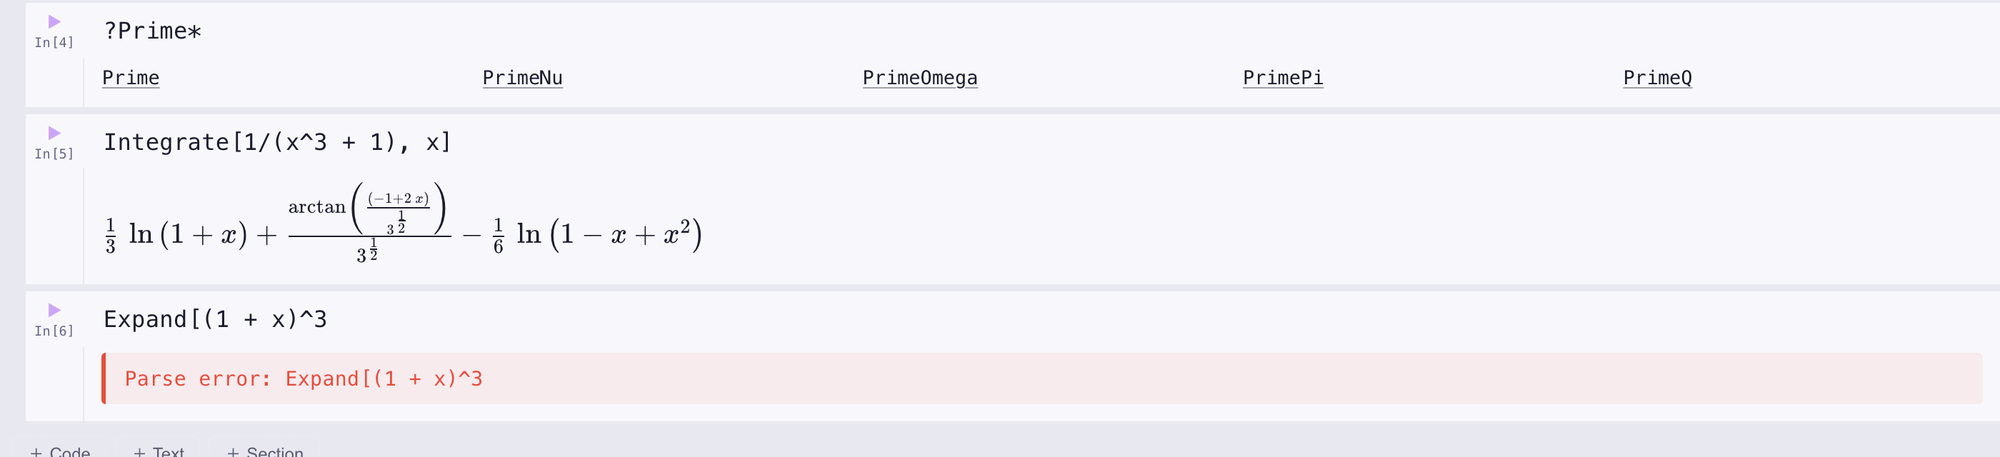
\includegraphics[width=\linewidth]{figures/notebook/names-error.png}
  \caption{A names grid from \texttt{?Prime*}, an indefinite integral, and a
  parse error. The error echoes the text the kernel received.}
  \label{fig:nb-names}
\end{figure}

An \mcode{error} is shown as a red block with the kernel's message
(Figure~\ref{fig:nb-names}). The same block is used when the evaluation itself
fails in the Rust layer, for example because the kernel process has died; in
that case the cell is marked as an error and the kernel as not running.

\subsection{Plots}
\label{ssec:nb-plots}

A \mcode{plot} message is drawn by Plotly, loaded the first time a plot
appears. Before drawing, the notebook overrides the figure's background, grid
and tick colours so that the plot matches the current theme. Everything else
comes from the kernel. Because Plotly draws the figure, the plot has Plotly's
own toolbar in its upper right corner, with zoom, pan, reset and a button
that saves a PNG, and you can drag a rectangle to zoom
(Figure~\ref{fig:nb-plot}). A \B{Plot3D} surface arrives as a
\mcode{Graphics3D} and is drawn as a Plotly 3D scene that turns under the
mouse.%
\calloutnote{Pitfall}{The theme is applied when the plot is drawn. Switching
between light and dark later does not redraw existing plots, so a plot made
in the dark theme keeps its dark background until you run its cell again.}

\begin{figure}[htbp]
  \centering
  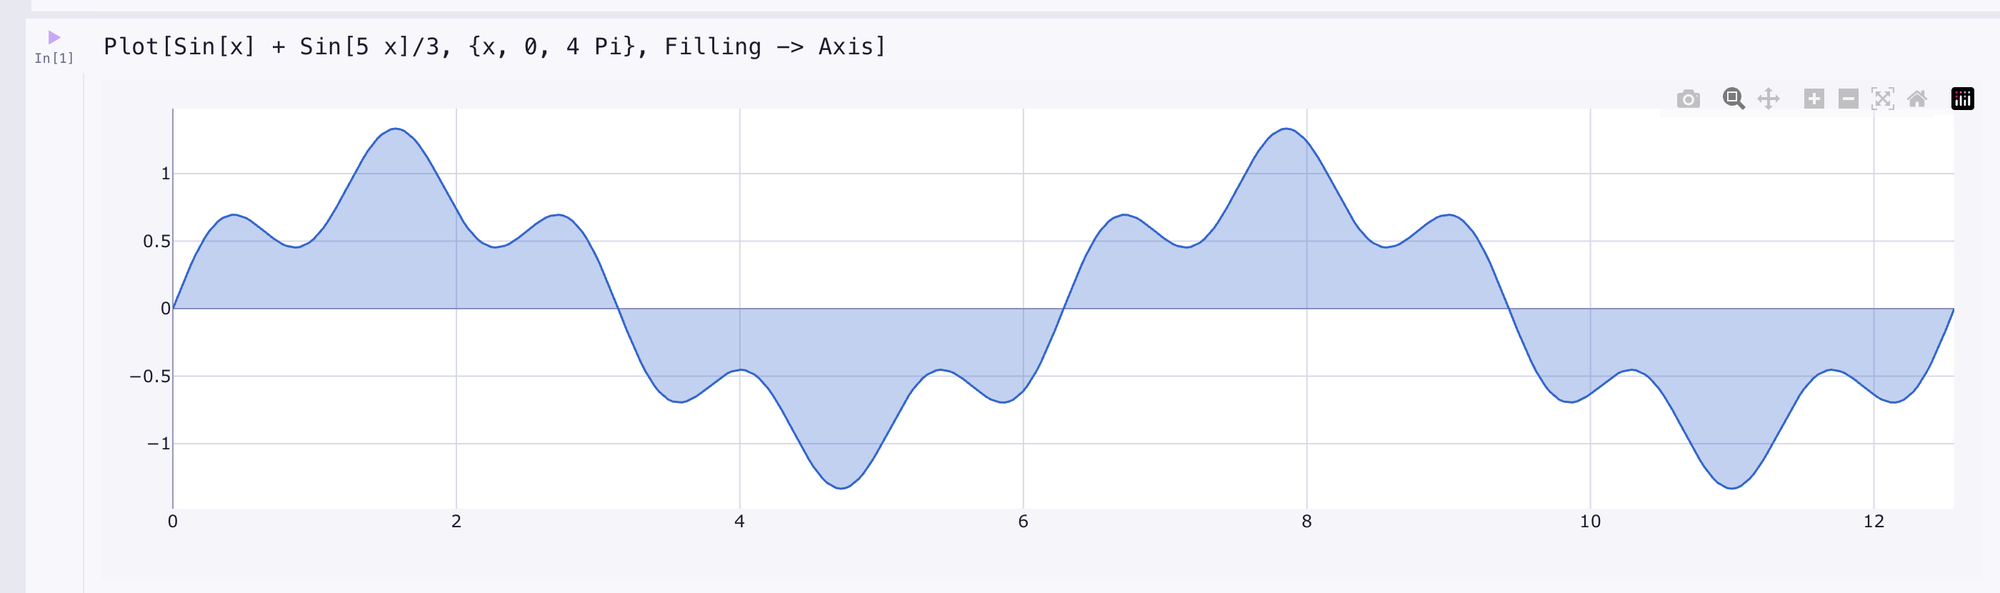
\includegraphics[width=\linewidth]{figures/notebook/plot.png}
  \caption{\texttt{Plot} with \texttt{Filling -> Axis}, drawn by Plotly from
  the kernel's figure. Plotly's toolbar is at the upper right.}
  \label{fig:nb-plot}
\end{figure}


\subsection{Images}
\index{notebook!images}

An \mcode{image} message is drawn on an HTML canvas at its natural pixel
size, and CSS scales the canvas to the display width with
\mcode{image-rendering: pixelated}. A three-by-three image therefore appears
as a visible grid of nine sharp squares. The kernel sends raw RGBA,
so the notebook copies the bytes straight into the canvas with
\mcode{putImageData} and no image file is ever encoded or decoded.

The default display width is chosen so that small images are visible and
large ones fit. A width \(w\) under 64 pixels is magnified twelve times, and
the result is then clamped between 48 and 512 pixels:
\[
  \text{shown width} = \min\bigl(\max(w\cdot m,\ 48),\ 512\bigr),
  \qquad m = \begin{cases} 12 & w < 64\\ 1 & w \ge 64. \end{cases}
\]
A note under each image gives its size, for example \mcode{128×128}, and the
channel count when there is more than one.

Click an image to select it. A frame appears with a mark at each of its four
corners. Drag any corner outward to enlarge the image and inward to shrink
it; the height follows the width, so the aspect ratio cannot be distorted by
accident. Once an image is selected you can also drag anywhere on it to
resize. Double-click a corner, or the selected image, to go back to the
default width. The note under the image then reports the size it is shown at
(Figure~\ref{fig:nb-image}). Clicking anywhere outside an image clears the
selection.%
\calloutnote{Performance}{A resize drag does not change any Svelte state
while it is in progress. An earlier version updated the stored width on
every mouse movement, which re-rendered the whole output list and reflowed
the page around it; on a reference page with sixty examples the resize
visibly lagged the pointer. Now the drag writes the width directly onto the
one element that changes, at most once per animation frame, and stores the
final width when you release the button. The same rule applies to turning a
volume. The width is kept per output and is never written into the notebook,
because a display size is a way of looking at a result and not part of it.}

\begin{figure}[htbp]
  \centering
  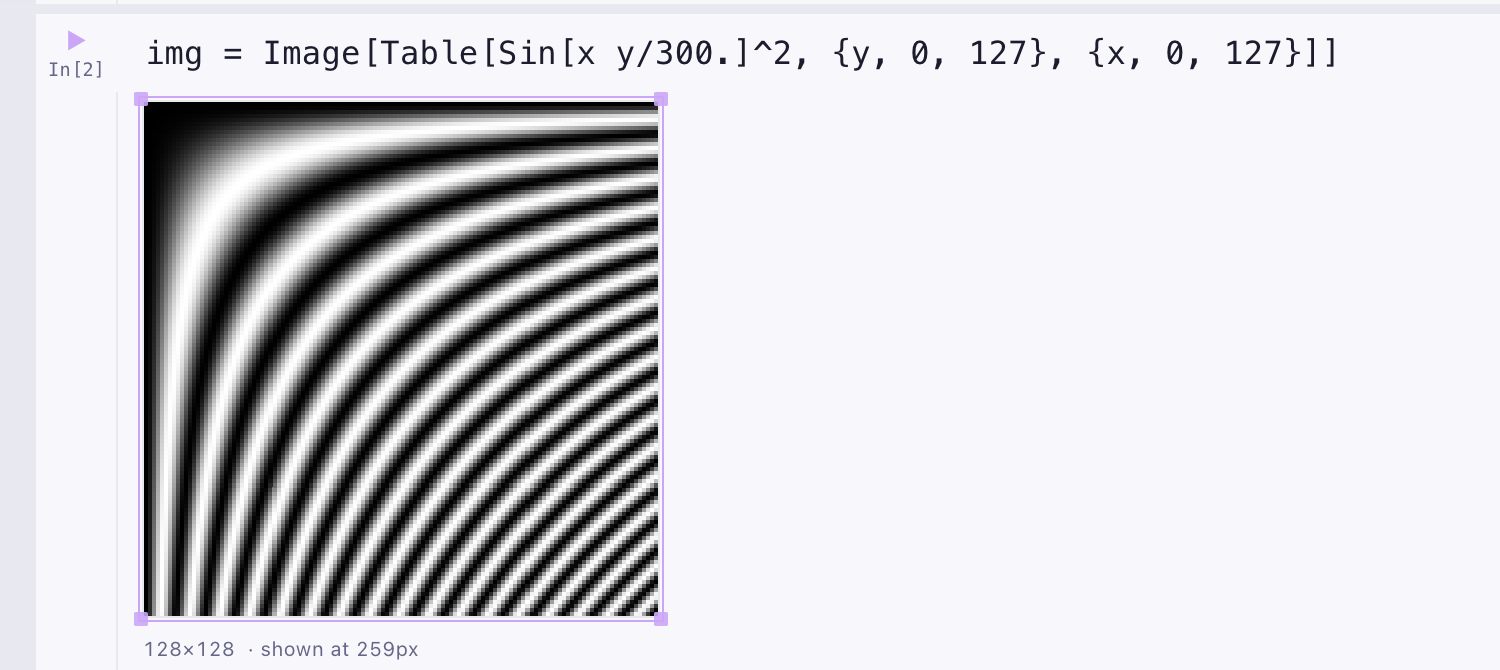
\includegraphics[width=0.75\linewidth]{figures/notebook/image-resized.png}
  \caption{A \(128\times128\) image, selected and dragged from its lower right
  corner. The note reports the new display width. The corner marks show only
  while the image is selected.}
  \label{fig:nb-image}
\end{figure}


\subsection{Volumes}
\label{ssec:nb-volumes}
\index{notebook!Image3D volumes}

An \mcode{Image3D} is a block of voxels, and one slice of it says little
about its shape. The notebook draws a volume as a shaded box that you turn by
dragging, much as Mathematica does. To make that possible the kernel sends
more than one slice. The message for a volume carries \mcode{depth},
\mcode{slice} (the 1-based index of the middle slice, which is also sent as
\mcode{data} for any consumer that can only show a flat image), and an
object \mcode{faces} with six entries named \mcode{front}, \mcode{back},
\mcode{left}, \mcode{right}, \mcode{top} and \mcode{bottom}. Each face is a
small RGBA image of its own, at most 256 pixels on a side.

A box seen from any direction shows at most three of its faces, so six
images are everything the renderer needs. For a \(256^3\) volume that is
\(6 \times 65\,536\) samples instead of 16.7 million. The interesting
question is what to put on a face.%
\calloutnote{Theory}{A face is a \emph{projection through} the volume along
one axis, composited front to back in the emission--absorption model used in
volume rendering. Along each ray, with voxel luminance \(v\), per-sample
opacity \(a = vK\), accumulated colour \(C\), accumulated alpha \(A\) and
remaining transmittance \(T\) (starting at 1),
\[
  C \leftarrow C + v\,a\,T,\qquad
  A \leftarrow A + a\,T,\qquad
  T \leftarrow T\,(1-a).
\]
The constant \(K = 4/L\) scales with the ray length \(L\), so that a path of
unit-valued voxels a quarter of the way through the volume reaches about 63\%
opacity whatever the volume's depth. The loop stops once \(T < 0.003\). The
colour is then divided by \(A\), and \(A\) itself becomes the face's alpha
channel, so empty space stays transparent. A voxel's own alpha channel, when
the volume has one, scales its contribution.}

The first version put only the outermost layer of voxels on each face, on
the reasoning that an opaque box shows only its surface. The comment in
\texttt{image.c} records why that failed. A ball with empty space on every
side has only zeros on its boundary, so \B{GaussianFilter}, \B{Dilation} and
\B{MeanFilter} applied to a ball all rendered as the same black hexagon.
With projections, each face shows what you would see looking into the volume
from that side, and the three results look different.

\begin{figure}[htbp]
  \centering
  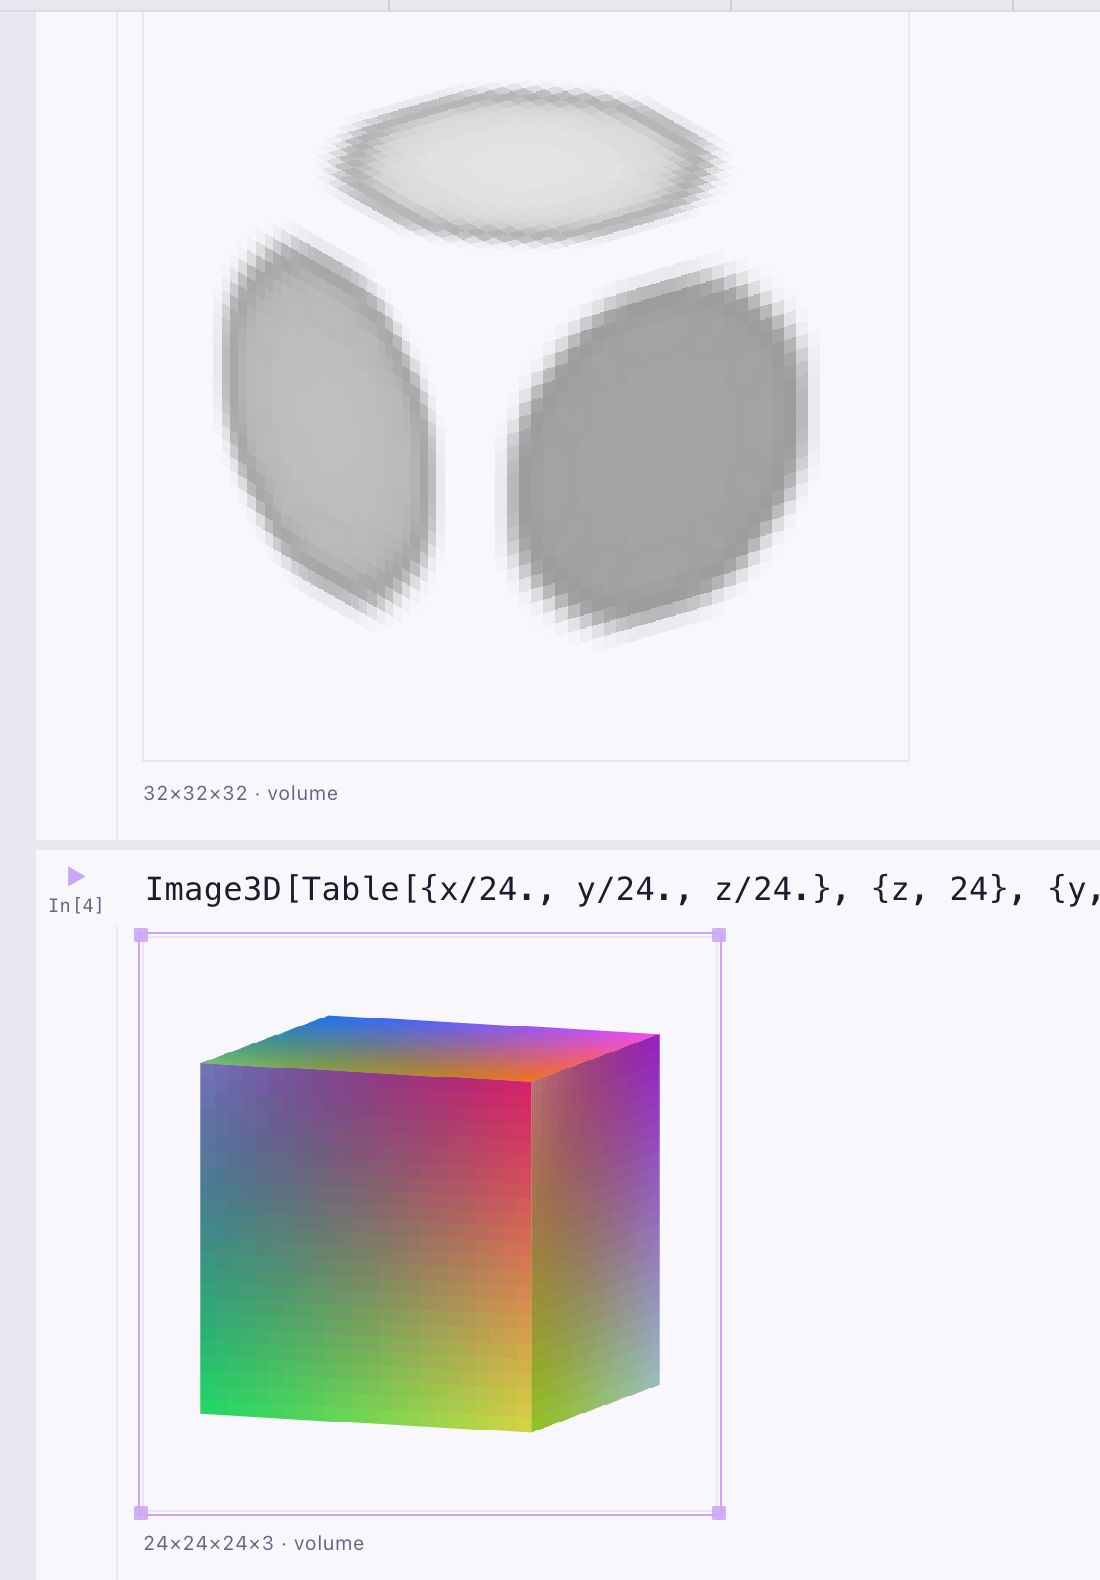
\includegraphics[width=0.55\linewidth]{figures/notebook/volumes.png}
  \caption{Two volumes. Above, a blurred ball: each visible face carries the
  ball's projection, and the transparent corners let the three discs show as
  separate shapes. Below, a \(24^3\) colour cube whose voxel colours are its
  own coordinates, turned by dragging and currently selected.}
  \label{fig:nb-volumes}
\end{figure}

The notebook draws the box with an orthographic camera. Under an
orthographic projection, the image of a flat rectangle is an \emph{affine}
image of it, so each face can be drawn by one call that sets a
\(2\times3\) transformation matrix and paints the face's texture. No
triangles are needed and no WebGL. For each face the renderer rotates the
face's corners by the current yaw and pitch, keeps the faces whose normal
points toward the viewer, sorts them from back to front, darkens each
according to the angle between its normal and a fixed light from the upper
left, and draws it. The darkening is applied only where the texture is
opaque, so a transparent region stays transparent. The box keeps the
volume's proportions: a \(4\times4\times32\) volume is drawn as a column.

Drag on the volume to turn it. Horizontal movement changes the yaw and
vertical movement the pitch, and the pitch stops just short of straight up
or down, where the box would collapse to a line. Double-click to return to
the default three-quarter view. The corner marks resize a volume exactly as
they resize an image. The note under a volume reads, for example,
\mcode{32×32×32 · volume}. If the kernel could not build the faces it sends
the middle slice alone, and the note says which slice is shown.

\section{Editing and the keyboard}
\label{sec:nb-keyboard}
\index{notebook!keyboard shortcuts}

Input cells are CodeMirror editors with CodeMirror's standard key bindings
and undo history. The editor knows Mathilda's comment syntax,
\mcode{(* \ldots{} *)}, so \emph{Un/Comment Selection} works; it does not
install a Mathilda language mode, so there is no syntax highlighting and no
automatic bracket closing. The keys that matter most are listed in
Table~\ref{tab:nb-cellkeys}.

\begin{table}[htbp]
\centering
\small
\begin{tabular}{@{}p{0.34\linewidth}p{0.58\linewidth}@{}}
\toprule
\textbf{Key} & \textbf{Action} \\
\midrule
\multicolumn{2}{@{}l}{\emph{In a code cell}}\\
\texttt{Shift+Enter} & Evaluate the cell. \\
\texttt{Cmd+Enter} & Evaluate the cell and insert an empty code cell below it. \\
\texttt{Up} on the first line & Leave the cell; show the insertion bar above it. \\
\texttt{Down} on the last line & Leave the cell; show the insertion bar below it. \\
\texttt{Cmd+Z}, \texttt{Cmd+Shift+Z} & Undo and redo within the cell. \\
\midrule
\multicolumn{2}{@{}l}{\emph{In a text cell or heading}}\\
\texttt{Up} at the start, \texttt{Down} at the end & Leave the cell, as above. A heading leaves at once. \\
\midrule
\multicolumn{2}{@{}l}{\emph{At the insertion bar}}\\
\texttt{Up}, \texttt{Down} & Enter the nearest editable cell in that direction. \\
\texttt{Enter} & Insert an empty code cell at the bar. \\
any printable key & Insert a code cell at the bar that starts with that character. \\
\texttt{Escape} & Hide the bar. \\
\midrule
\multicolumn{2}{@{}l}{\emph{Anywhere}}\\
\texttt{F1} or \texttt{Cmd+I} & Open the reference page for the symbol at the caret. \\
\texttt{Cmd}+click on a name & Open that symbol's reference page. \\
\texttt{Cmd+F} & Find across every cell (focused mode). \\
\texttt{Cmd+=}, \texttt{Cmd+-} & Scale the interface up or down by 10\%, between 50\% and 200\%. \\
\texttt{Cmd+0} & Reset the scale to 100\% and fit all cards in the window. \\
\texttt{Cmd+\textbackslash} & Split the window with the next notebook, side by side. \\
\texttt{Cmd+Shift+\textbackslash} & The same split, stacked. \\
\texttt{Cmd+S}, \texttt{Cmd+O} & Save and open the library (\S\ref{sec:nb-files}). \\
\bottomrule
\end{tabular}
\caption{Keys handled by the web view. \texttt{Ctrl} works wherever
\texttt{Cmd} is shown. The native menu adds its own accelerators
(Table~\ref{tab:nb-menus}).}
\label{tab:nb-cellkeys}
\end{table}

\paragraph{Moving between cells.} The arrow keys walk through the notebook
as a single document.\index{notebook!insertion bar} Pressing Down on the last
line of a cell shows a thin \emph{insertion bar} in the gap below, and a second Down enters the next cell
at its first line. Pressing Enter at the bar inserts a new code cell there,
and typing any character inserts a code cell that begins with it, which is
the quickest way to add a cell between two others. Cells the caret cannot
enter are stepped over: the read-only prose and headings of a reference page
do not stop the caret, so arrowing through documentation moves from one
example to the next. Each cell that takes the caret scrolls itself into view,
and only when it is actually off screen, so a short step does not jolt the
page.

\paragraph{Cell operations.} The toolbar's \emph{Cells} group splits the
active cell at the caret, merges it with the cell below, duplicates it, and
deletes it. A split keeps the text before the caret and moves the rest into
a new cell of the same type directly below; if the caret position is not
available, the split happens at the end and produces an empty cell. A merge
joins the two sources with a newline, never by concatenation, because two
code cells mean two statements. A duplicate copies the source only. It does
not copy the output, since the copy has not been evaluated. Deleting the last
cell of a notebook leaves one empty code cell behind. The \emph{Code} group,
shown while a code cell is active, indents, outdents, duplicates the current
line, and comments or uncomments the selection.

\paragraph{Templates.} While a code cell is active, the \emph{Insert} group
offers fourteen templates: Table, a two-by-two matrix, Sum, Product,
Integrate, NIntegrate, Derivative, Limit, Solve, Plot, Module, a function
definition, Replace all, and Map (Figure~\ref{fig:nb-insert}). Each menu entry
shows what it will insert. A template lands at the caret with named
placeholders, and Tab moves from one placeholder to the next.%
\calloutnote{Under the hood}{A template with an unbalanced bracket would
insert a broken cell every time it was used. The script
\texttt{npm run check:snippets} expands each template and passes the result
to the real Mathilda binary wrapped in \B{Hold}, which parses the text
without evaluating it, so the check cannot draw a plot or define a function.
A template that does not parse fails the check. The script also counts each
kind of bracket, because the parser says only that a line is wrong while a
count says which bracket is missing. If the binary has not been built, the
parser half reports SKIP.}

\begin{figure}[htbp]
  \centering
  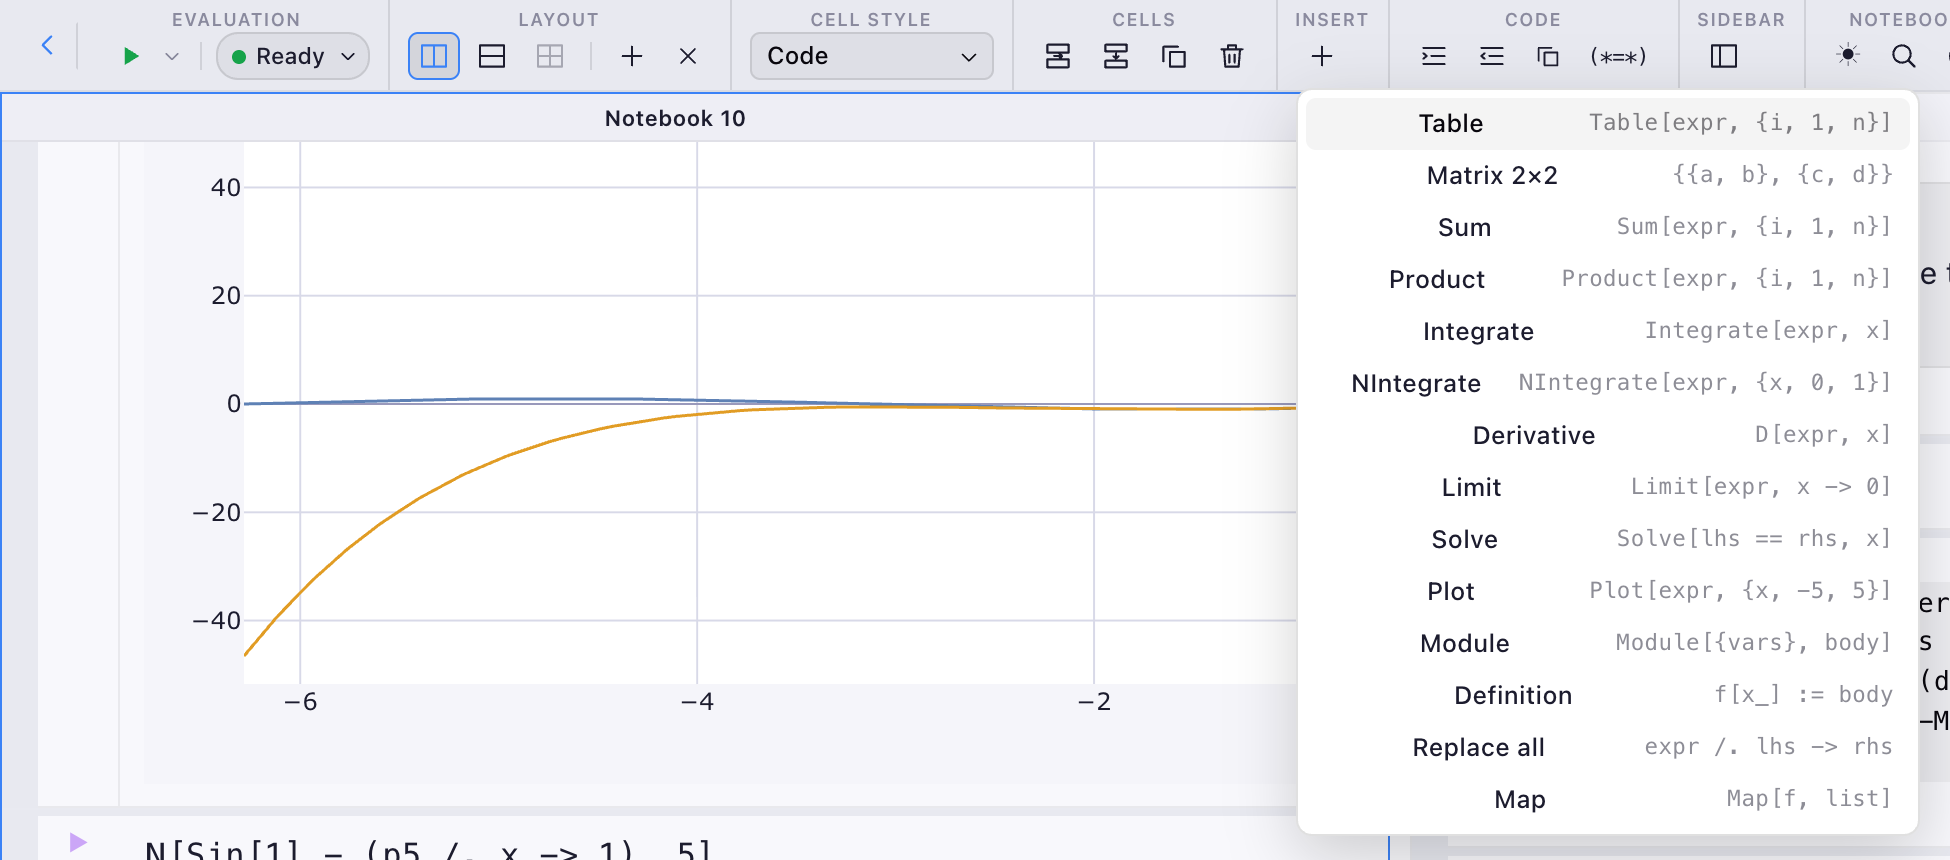
\includegraphics[width=0.8\linewidth]{figures/notebook/insert-menu.png}
  \caption{The Insert palette. The hint beside each name is the exact text
  that the template inserts, before any placeholder is filled in.}
  \label{fig:nb-insert}
\end{figure}


\paragraph{Find.} \texttt{Cmd+F} in focused mode searches every cell of the
active notebook, code and prose, and reports the position as \emph{n of m}.
Typing only updates the count; Enter jumps to the next match and Shift+Enter
to the previous one, wrapping at both ends. In a code cell the match is
selected in the editor and scrolled into view; a text cell is opened for
editing and its match selected. Matches never overlap, so \mcode{aa} occurs
twice in \mcode{aaaa}. There is no highlighting of all matches at once.%
\calloutnote{Pitfall}{Jumping to a match moves keyboard focus into the cell
that holds it, so that the selection is live. A second press of Enter then
goes to that cell, where it replaces the selected match with a newline.
Use the arrow buttons in the find bar to step through further matches, or
click back into the search field before pressing Enter again.}

\section{Menus and the toolbar}
\label{sec:nb-menus}
\index{notebook!menus}

On macOS the notebook's menus live in the system menu bar at the top of the
screen, which leaves the window's own top strip free for the toolbar.
Table~\ref{tab:nb-menus} lists the menus and their accelerators. Undo, redo,
cut, copy, paste and select all are the system's predefined items, so they
reach the focused editor through the normal macOS route and behave exactly
as they do in any Mac application.

\begin{table}[htbp]
\centering
\small
\begin{tabular}{@{}lp{0.5\linewidth}p{0.3\linewidth}@{}}
\toprule
\textbf{Menu} & \textbf{Items} & \textbf{Accelerators} \\
\midrule
File & New Notebook, Open, Save, Save As, Print, Close Notebook, Close Window
  & \texttt{Cmd+N}, \texttt{O}, \texttt{S}, \texttt{Shift+S}, \texttt{P}, \texttt{W} \\
Edit & Undo, Redo, Cut, Copy, Paste, Select All; Un/Comment Selection;
  Indent and Outdent Selected Lines; Duplicate Line; Documentation for Selection
  & \texttt{Cmd+/}, \texttt{Cmd+Shift+L}, \texttt{Cmd+Shift+F} \\
Insert & Input Cell, Text Cell, Section Cell & \texttt{Cmd+B} (Input) \\
Cell & Convert to Input, Text or Section; Divide, Merge, Duplicate, Delete;
  Delete Output, Delete All Output & \texttt{Cmd+Shift+D}, \texttt{Cmd+Shift+M} \\
Evaluation & Evaluate Cell, Evaluate Notebook, Abort Evaluation, Restart Kernel
  & \texttt{Cmd+Return}, \texttt{Cmd+Shift+Return}, \texttt{Cmd+.}, \texttt{Cmd+Shift+R} \\
Graphics & Plot, Image, Image3D and Graphics documentation & \\
View & Toggle Dark Mode & \texttt{Cmd+Shift+T} \\
\bottomrule
\end{tabular}
\caption{The native menu bar (desktop only).}
\label{tab:nb-menus}
\end{table}

Each native item has an id, such as \mcode{cell.merge}. When you choose it,
Rust emits an event named \mcode{menu:cell.merge}, and a dispatcher in
\texttt{menuCommands.ts} runs the matching command against the active pane.
The list of ids is exported from that file and is the list the web view
subscribes to, so an item added in Rust without a handler produces a console
warning instead of silently doing nothing. The toolbar's buttons call the
same functions, so the menu and the toolbar cannot drift apart.

\emph{Close Notebook} (\texttt{Cmd+W}) closes the notebook in the active
pane, and \emph{Close Window} closes the window. The first is on the more
familiar key because it is the one you use repeatedly. The Graphics menu is a
set of documentation entry points, because plots have no editable object
model for drawing tools to act on. \mcode{Graphics} itself has no reference
page yet, so its item opens a card saying so. \emph{Documentation for Selection} opens
the page for the selected word; with nothing selected it opens the \B{Image}
page, which is the subsystem the current startup content documents.%
\calloutnote{Pitfall}{In the build examined for this chapter, the three
\emph{Convert to} items in the Cell menu update only the toolbar's record of
the active cell's type. They do not change the cell itself. Use the toolbar's
\emph{Cell Style} control to change a cell's type, or the type badge in the
gutter of a text or heading cell. The source of this discrepancy is the
function \texttt{retypeActiveCell} in \texttt{active.ts}, which the menu calls
on its own while the toolbar calls it after changing the store.}

\subsection{The toolbar}

Focused mode replaces the card's title bar with a toolbar of labelled
groups. From left to right:

\begin{description}
\item[Back] Return to the canvas. This button is never hidden, because it is
  the only way back that works with a plain mouse; the other is a pinch-out
  gesture on a trackpad.
\item[Evaluation] A Run button that evaluates the active code cell, or the
  whole notebook when no code cell is active; a menu with \emph{Evaluate
  cell}, \emph{Evaluate notebook}, \emph{Evaluate from here down} and
  \emph{Evaluate above} (Figure~\ref{fig:nb-evalmenu}); and the kernel status
  with a menu offering \emph{Abort evaluation (restarts kernel)} and
  \emph{Restart kernel}.
\item[Layout] Side by side, stacked, two-by-two grid, add a pane, remove the
  active pane.
\item[Cell Style] The type of the active cell, as a menu. With no active cell
  it reads \emph{Insert Cell\ldots} and inserts a new cell of the chosen type.
\item[Cells] Split, merge, duplicate, delete.
\item[Insert] and \textbf{Code} For code cells only (\S\ref{sec:nb-keyboard}).
\item[Text] For text cells only (\S\ref{sec:nb-text}).
\item[Sidebar] Show or hide the properties panel.
\item[Notebook] Theme, find, and a documentation menu with \emph{Documentation
  for} the symbol at the caret and \emph{Browse all symbols}.
\end{description}

\noindent The title of the active pane sits at the right end, followed by an
overflow menu with the input and output layout, fold-all, the status bar
toggle, rename, collapse and close. Groups that do not apply are hidden
entirely, so a row of dead controls never appears.%
\calloutnote{Under the hood}{Every toolbar button suppresses the default
action of the pointer-down event. Without that, clicking a button would move
focus out of the editor before the button's handler ran, and a command such
as \emph{Split at caret} would find no caret. The record of the active cell
is also never cleared on blur; it is only marked as unfocused, and every
toolbar reading looks the cell up again in its notebook, so a deleted cell or
a closed notebook reads as ``no active cell'' without any clean-up code.}

\begin{figure}[htbp]
  \centering
  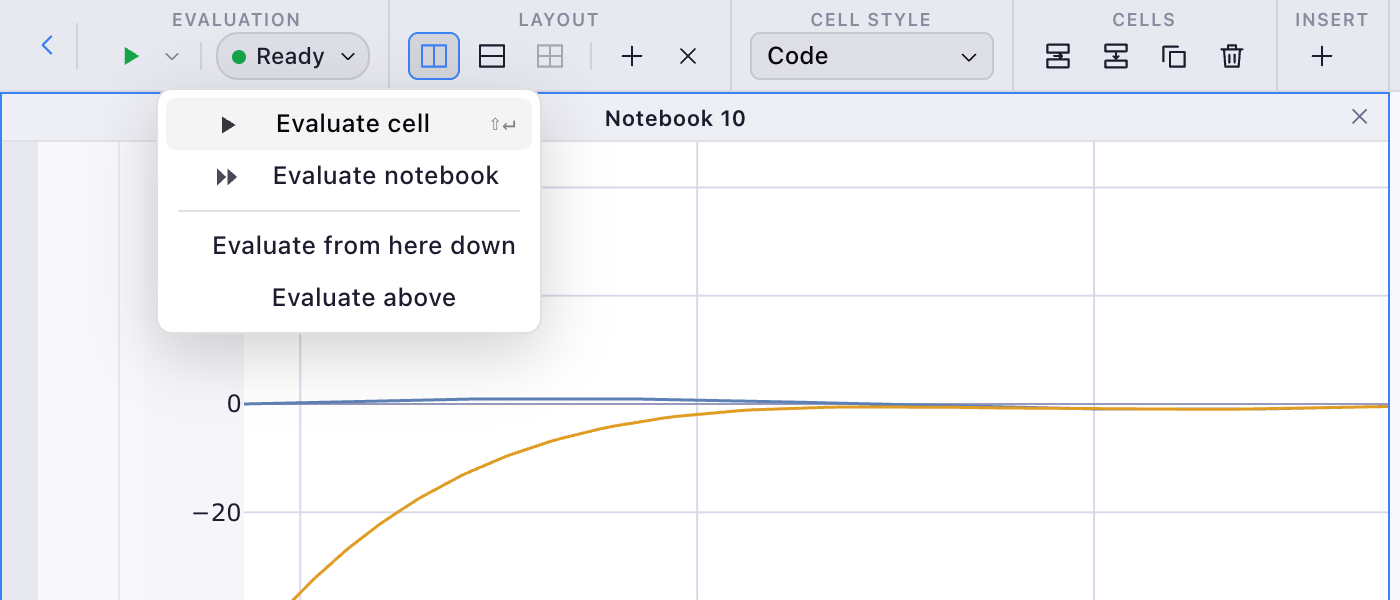
\includegraphics[width=0.62\linewidth]{figures/notebook/eval-menu.png}
  \caption{The Evaluation menu. \emph{Evaluate from here down} and
  \emph{Evaluate above} run a range of cells without renumbering the rest.}
  \label{fig:nb-evalmenu}
\end{figure}


\paragraph{Input beside output.} The overflow menu's \emph{Input and output
side by side} puts each code cell's result to the right of its input
(Figure~\ref{fig:nb-side}). A handle between the two columns can be dragged
to set the split between 15\% and 85\%. This suits a wide window and short
inputs.

\begin{figure}[htbp]
  \centering
  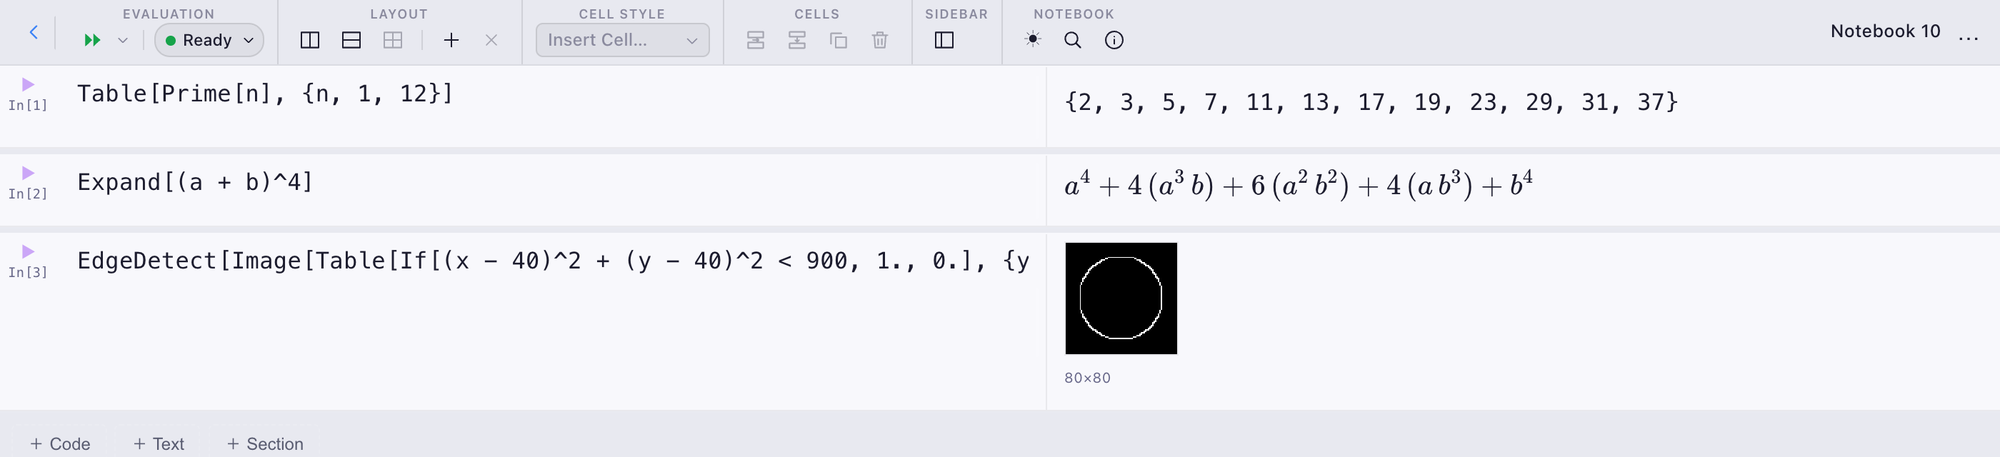
\includegraphics[width=\linewidth]{figures/notebook/side-by-side.png}
  \caption{Input and output side by side. The first result has more than four
  commas, so it is shown as wrapping text instead of typeset. The third is an
  \texttt{EdgeDetect} image.}
  \label{fig:nb-side}
\end{figure}

\section{The canvas, panes and documentation}
\label{sec:nb-docs}
\index{notebook!reference pages}

\paragraph{The canvas.} Two-finger scrolling pans the canvas and pinching
zooms it, centred on the pointer, between 8\% and 300\%. A scroll that starts
over a card scrolls the card while the card can still move in that direction.
When the card reaches its end, the rest of that flick is absorbed, so the
canvas does not suddenly fly away; pausing and scrolling again pans the
canvas. Dragging on empty canvas draws a selection rectangle, and dragging
any selected card moves them all. Double-click or right-click on empty canvas
to create a notebook there, press \texttt{N} to create one in the middle of
the view, or use the \emph{New Notebook} button at the bottom of the window.
With two or more cards selected, Enter or \texttt{Cmd+\textbackslash} opens
them together in focused mode, and buttons offer the side-by-side, stacked
and grid arrangements. Pinching out in focused mode returns to the canvas.

\paragraph{Panes.} Focused mode can show up to four notebooks at once. A
notebook can appear in only one pane, and the toolbar acts on the
\emph{active} pane, whose border is highlighted and whose title is shown at
the right of the toolbar. Clicking in a pane makes it active. Dividers
between panes can be dragged, and a two-by-two grid has two independent
dividers. Removing a pane leaves its notebook on the canvas; the close button
in the toolbar deletes the notebook itself. Figure~\ref{fig:nb-grid} shows a
working notebook tiled with three reference pages.

\begin{figure}[htbp]
  \centering
  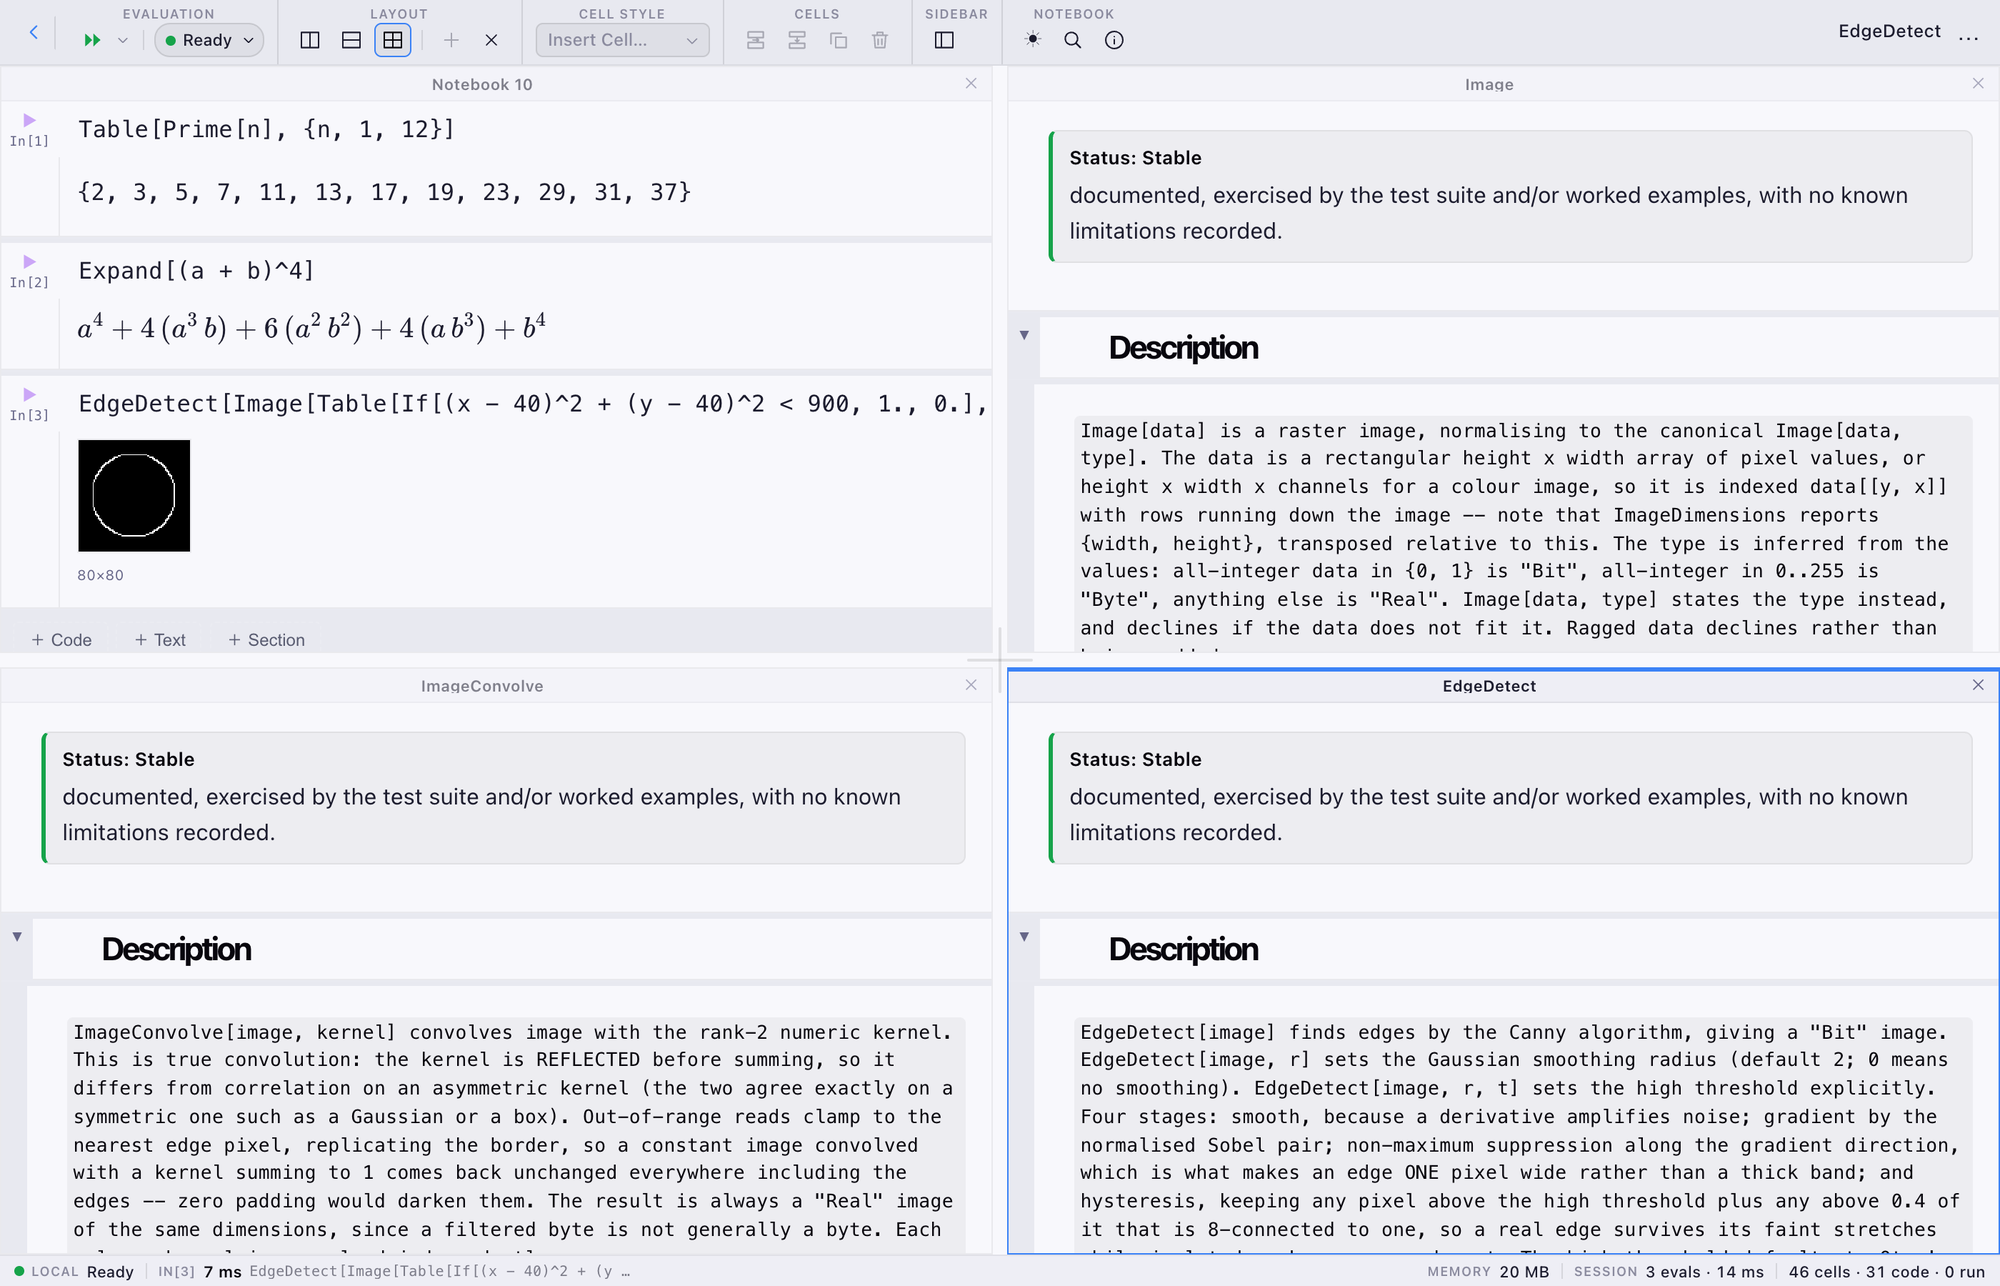
\includegraphics[width=\linewidth]{figures/notebook/grid.png}
  \caption{Four panes in a two-by-two grid: a working notebook and the
  reference pages for \texttt{Image}, \texttt{ImageConvolve} and
  \texttt{EdgeDetect}. The active pane has the blue border.}
  \label{fig:nb-grid}
\end{figure}

\paragraph{Documentation beside your work.} There are four ways to open a
symbol's reference page: press \texttt{F1} or \texttt{Cmd+I} with the caret
in the name, \texttt{Cmd}+click the name anywhere in the window, click the
\emph{Documentation} button under a usage message, or click a name in a names
grid. The gesture only claims names that have a page, so \texttt{Cmd}+click on
a variable behaves normally. On the canvas the page opens as a new card just
to the right of where you clicked. In focused mode it opens as a pane on the
right, and the caret stays in your own notebook, so your next
\texttt{Shift+Enter} still evaluates your own cell. Repeated lookups reuse
the documentation pane instead of adding a new pane each time
(Figure~\ref{fig:nb-docpane}).

\begin{figure}[htbp]
  \centering
  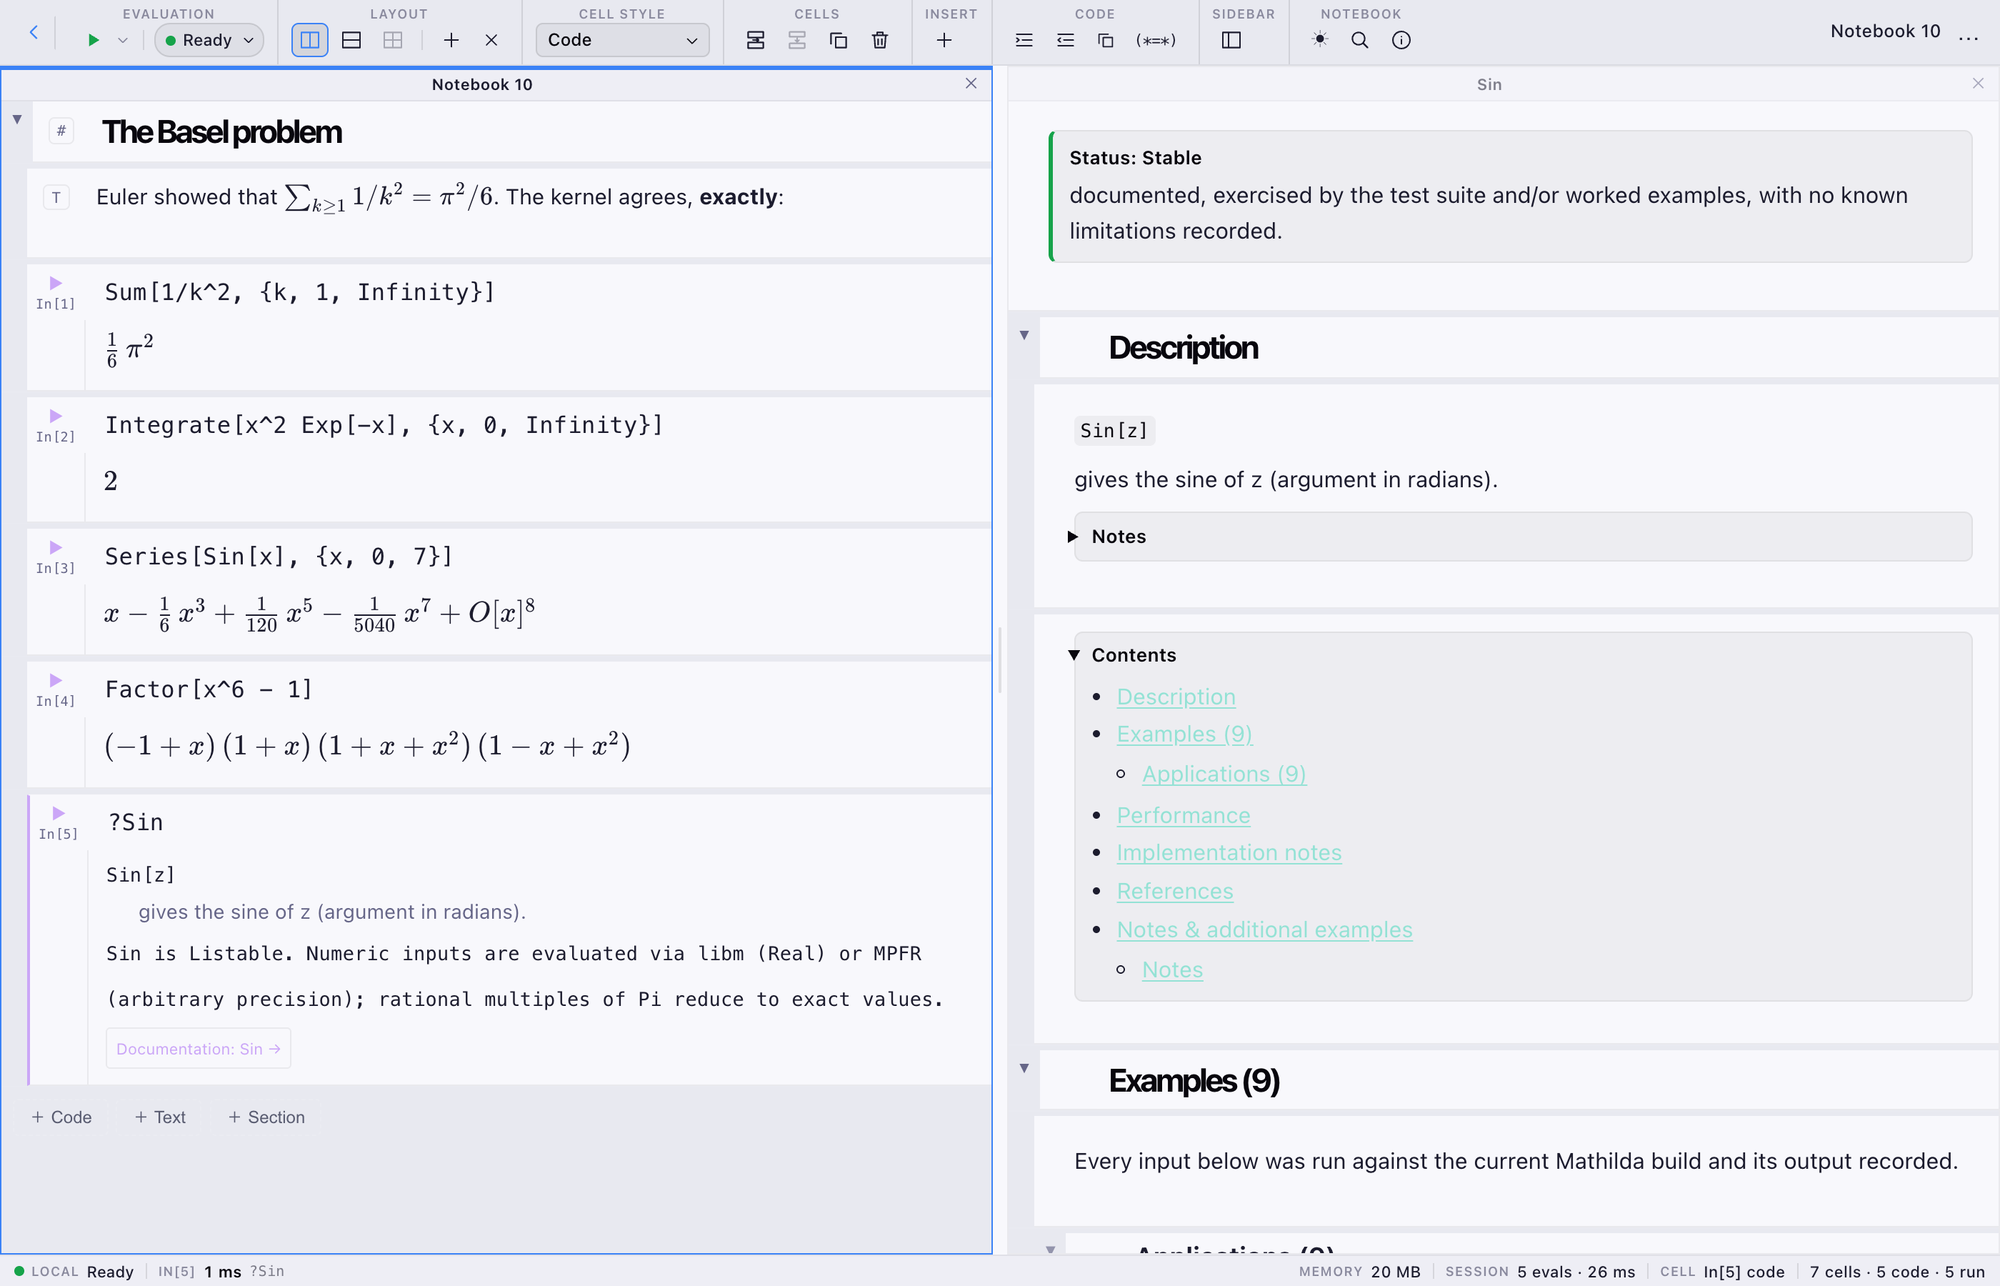
\includegraphics[width=\linewidth]{figures/notebook/docpane.png}
  \caption{The reference page for \texttt{Sin}, opened in a pane beside the
  notebook by the \emph{Documentation} button under \texttt{?Sin}. Each
  heading folds the section beneath it, and the contents list links to the
  sections.}
  \label{fig:nb-docpane}
\end{figure}

A reference page in the notebook is a real notebook. The pages are the
Markdown files generated for the website by \texttt{site/generate.py}, which
re-runs every example against the built binary. When the notebook opens a
page it splits the Markdown into cells. Each level-two or level-three heading
becomes a section or subsection cell, so every part of the page folds. Prose
becomes reference cells. Every \mcode{In[n]:=} example becomes a code cell
holding the input, with the recorded result shown underneath in plain
monospace until you run the cell. A recorded result is never typeset: it is
Mathilda text, and KaTeX would render something like
\mcode{Derivative[1][g][x]} as italic mathematics. Examples whose result is a
plot arrive with the saved Plotly figure, and examples whose result is an
image arrive with the recorded picture. Run any example and the live result
replaces the recording; edit it first and you are experimenting inside the
documentation. A table of contents is inserted after the Description section.%
\calloutnote{Under the hood}{The pages are copied into the app by
\texttt{scripts/sync-refpages.mjs}, which runs before every \texttt{npm run
dev} and \texttt{npm run build}. It builds an index from symbol name to file,
because names are not unique across categories: \B{Det}, \B{Factor} and a few
others are documented both in their own category and in the FLINT section,
and a flat copy would let one page overwrite the other. The index prefers the
category that the site's \texttt{builtins.json} assigns to the symbol, which
is the page the website links to. The pages are fetched with caching
disabled, because a cached page would silently show the previous build's
documentation.}

\section{The kernel's state and the status bar}
\label{sec:nb-kernel}
\index{notebook!kernel lifecycle}

The kernel is always in one of five states, shown by a coloured dot and a
word in the toolbar: Starting, Ready, Running, Restarting, and Not running.

\paragraph{Restart} kills the kernel and starts a fresh one. The Rust shell
first sends \mcode{quit}, waits 300 milliseconds, and kills the process. It
then tries up to three times to start a new one, waiting half a second before
the second attempt and a second before the third. A restart discards every
definition in the session, in every notebook, and resets the status bar's
session totals.

\paragraph{Abort} does the same thing.\index{notebook!abort} The kernel has no
way to stop an evaluation part way through, so the notebook stops a long
computation by killing the process and then restarts it. That is why the
menu item reads \emph{Abort evaluation (restarts kernel)}: you regain control
at the cost of the session's definitions. Pressing \texttt{Cmd+.} while
nothing is running does nothing, so a habitual keypress does not throw away a
healthy session. The source says plainly that a cooperative abort, a flag
checked inside the evaluator so that the computation stops and the state
survives, is the proper fix, and that it is kernel work.

\begin{figure}[htbp]
  \centering
  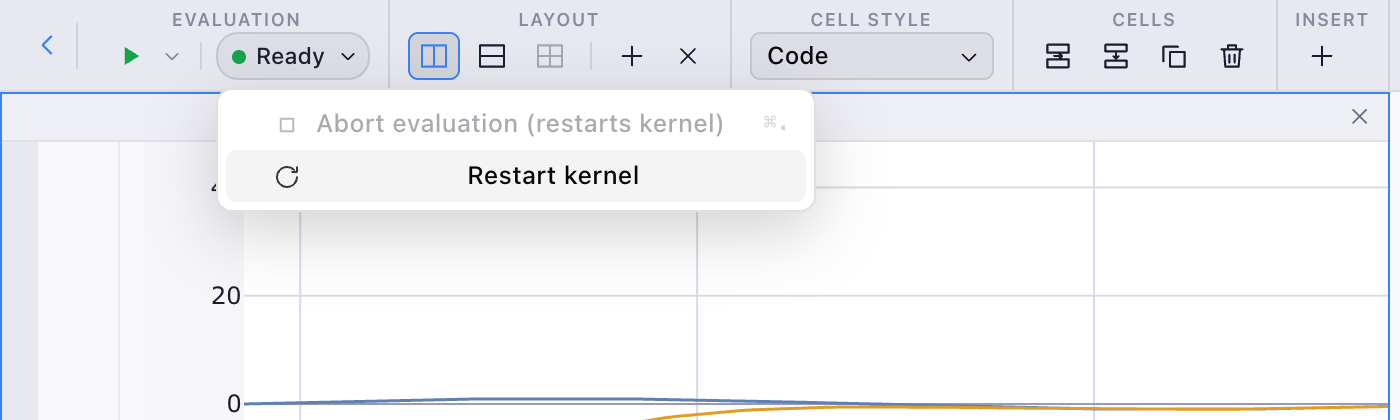
\includegraphics[width=0.62\linewidth]{figures/notebook/kernel-menu.png}
  \caption{The kernel menu. The abort item says what it costs.}
  \label{fig:nb-kernelmenu}
\end{figure}

\paragraph{The status bar} runs along the bottom of focused mode and can be
hidden from the overflow menu. From left to right it shows the kernel state
(click it to restart when the kernel is not running), the last evaluation
with its \mcode{In[n]} label, its duration and the first 42 characters of its
input, the kernel's memory as reported by the last \mcode{done} message, the
number of evaluations in this session and their total time, the type and
label of the active cell, and counts of cells, code cells and evaluated
cells. The duration is wall-clock time from the request to the last message,
measured with the browser's monotonic clock. It therefore includes any wait
for another pane's evaluation to finish.

\paragraph{The properties panel} slides in from the left when you press the
Sidebar button. It shows the notebook's name, its location, its size in
characters of source, cell counts, the kernel state with Restart and Abort
buttons, a dark-theme switch and the \emph{Show In[n] labels} switch, the interface
scale in steps of 75\%, 100\%, 125\% and 150\%, and the pane layout. The
Location row reads \emph{Not saved to a file} (or \emph{Generated reference
page}), because a notebook on the canvas has no file of its own
(\S\ref{sec:nb-files}). None of these
preferences is saved when the app quits.%
\calloutnote{Pitfall}{In the build examined for this chapter, both the
properties panel and the find bar are stacked beneath the focused-mode view:
their CSS \texttt{z-index} values are 40 and 45, and the view's is 50. Both
open, and both work, but neither can be seen, which is why this chapter has
no picture of either. Raising the two values above 50 would fix it.}

\section{Saving your work}
\label{sec:nb-files}
\index{notebook!file format}

\texttt{Cmd+S} saves the whole canvas, every notebook on it, as one
\emph{library} file with the extension \texttt{.lb}. \texttt{Cmd+O} opens a
library and replaces the canvas with it. The first save asks for a file name,
and later saves write to the same file. A library is JSON, written with
two-space indentation by \mcode{serializeLibrary} in \texttt{canvas.ts}. Its
shape is

\begin{shell}
{
  "version": "1",
  "type": "mathilda-library",
  "title": "Basel",
  "notebooks": [
    {
      "id": "nb-10",
      "title": "Notebook 10",
      "x": 520, "y": 240, "width": 640, "collapsed": false,
      "rows": [
        { "cells": [ { "type": "section", "source": "The Basel problem" } ] },
        { "cells": [ { "type": "code", "source": "Sum[1/k^2, {k, 1, Infinity}]" } ] }
      ]
    }
  ]
}
\end{shell}

\noindent (the listing is abbreviated; a real file lists every notebook and
every row). Only the source of each cell is saved, together with each card's
position, width and collapsed state. Outputs are not saved. A library
therefore diffs cleanly under version control and stays small, and opening
it shows every input with no results until you evaluate. A card's height,
the zoom and pan of the canvas, the pane layout, and whether a card was a
reference page are not saved either.

The Rust layer also contains a second, simpler format, written for single
notebooks. In it each cell is a stanza that begins with a comment line such
as \mcode{(* cell: code *)}, so a file of code cells is also a valid Mathilda
script. The commands \mcode{save\_notebook} and \mcode{load\_notebook}
implement it, and the project README describes it, but no menu item or
button in the current front end calls them. The Open dialog lists the
\texttt{.mathilda} extension, yet it reads every file as a library, so
opening a stanza file fails.%
\calloutnote{Pitfall}{\emph{Print\ldots} prints the web view through the
system print dialog. No command writes a notebook, with its outputs, to PDF
or HTML. To keep a picture of a plot, use
the camera button in Plotly's toolbar, which saves a PNG.}

\section{Building and running the notebook}
\label{sec:nb-build}
\index{notebook!building}

The notebook needs the Rust toolchain, Node.js~18 or later, the Tauri
command-line tool, and the same GMP and Readline libraries the kernel needs
(Chapter~\ref{ch:building}). From the repository root:

\begin{shell}
$ cd frontend
$ ./build-sidecar.sh          # build ./Mathilda and install it as the sidecar
$ npm install                 # JavaScript dependencies
$ cargo tauri dev             # run with hot reload
\end{shell}

\noindent \texttt{cargo tauri dev} runs \texttt{npm run dev}, which copies
the reference pages and starts the Vite development server, and then opens
the app. After you change the C kernel, run \texttt{build-sidecar.sh} again;
it refreshes the copy that the running development build uses. For a
distributable application:

\begin{shell}
$ ./build-sidecar.sh
$ cargo tauri build           # bundles land in src-tauri/target/release/bundle/
\end{shell}

The reference pages come from the website's generated documentation. If you
add a builtin, regenerate the site with \texttt{python3 site/generate.py} and
then run \texttt{npm run sync:refpages}, or the new symbol's page will be
missing from the app. Three small test scripts exercise the front end's pure
logic by compiling the real TypeScript modules and importing the result:
\texttt{npm run check:prose} (39 checks of Markdown and math rendering),
\texttt{npm run check:search} (18 checks of matching and wrap-around), and
\texttt{npm run check:snippets} (the template check described above).

\subsection{iOS and Android}
\label{sec:nb-mobile}
\index{notebook!mobile}

iOS and Android do not let an app start a child process, so on those systems
the kernel is compiled into a static library, \texttt{libmathilda.a}, and
linked into the app. The Rust module \texttt{kernel\_ffi.rs} replaces
\texttt{kernel.rs} at compile time with the same interface, so the rest of the
app is unchanged. The runbooks \texttt{frontend/IOS.md} and
\texttt{frontend/ANDROID.md} give the cross-compilation steps; iOS needs the
full Xcode, and Android needs API level 26 or later.

\begin{sloppypar}
The in-process kernel is more limited. Each evaluation calls one C function,
\mcode{mathilda\_ffi\_eval\_json}, which returns a single message: an
expression with its \LaTeX{}, a Plotly figure, or an error. It does not
produce image, usage or names messages. Restart and abort do nothing, because
a C call cannot be interrupted from another thread and the symbol table has
no reset function yet. The mobile kernel is built without FLINT, ECM and
LAPACK. On a touch screen, one finger pans the canvas and two fingers pinch
to zoom, and cards cannot be dragged or resized by touch.
\end{sloppypar}

\subsection{How the screenshots in this chapter were made}
\label{sec:nb-screenshots}

A book cannot show a native window without a screenshot, and a screenshot
staged by hand could show something the program does not do. The pictures in
this chapter were made by a script instead. It builds the web view with
\texttt{npm run build}, opens the result in headless Chrome, and replaces the
Tauri bridge with a small shim whose \mcode{evaluate\_cell} writes the same
JSON request that \texttt{kernel.rs} writes to a real \texttt{./Mathilda}
process in pipe mode, and passes each reply to the channel, dropping non-JSON
lines exactly as the Rust shell does. The script then types into cells,
clicks toolbar buttons, and drags corners and volumes like a user. Everything
drawn is the shipped front end rendering real kernel output. What the method
cannot show is the native part of the window: the macOS menu bar, the title
bar, and the file dialogs.

\section{Featured workflows}
\label{sec:nb-featured}

The vignettes below each describe one small, complete job, in the spirit of
the ``New in Version'' examples that Wolfram publishes for each Mathematica
release. Each uses only features that the front-end source supports.

\subsection*{Build a Report with Text and Math Cells}

A short derivation reads better with its argument in words beside it. Add a
section cell for the title, a text cell for the claim, and code cells for the
evidence:

\begin{shell}
Euler showed that $\sum_{k\ge 1} 1/k^2 = \pi^2/6$. The kernel agrees, **exactly**:
Sum[1/k^2, {k, 1, Infinity}]
\end{shell}

\noindent The text cell renders its formula with KaTeX as soon as you click
away, and the code cell's answer is typeset from the kernel's own \LaTeX{}
(Figure~\ref{fig:nb-report}). Save with \texttt{Cmd+S}: the library keeps the
prose and the inputs, and a colleague who opens it re-derives every result
with \emph{Evaluate notebook}.

\subsection*{Explore a Function Interactively}

To see how well a Taylor polynomial approximates the sine, compute the
polynomial once and reuse it:

\begin{shell}
p5 = Normal[Series[Sin[x], {x, 0, 5}]]
Plot[{Sin[x], p5}, {x, -2 Pi, 2 Pi}]
N[Sin[1] - (p5 /. x -> 1), 5]
\end{shell}

\noindent Each line is its own cell. The plot is a live Plotly figure: drag a
rectangle around the origin to zoom in and watch the two curves agree, then
double-click to zoom out and watch the polynomial run away beyond
\(|x| \approx 3\) (Figure~\ref{fig:nb-explore}). Change the 5 to 9 in the
first cell and choose \emph{Evaluate from here down} from the Evaluation menu
to redo the rest.

\begin{figure}[htbp]
  \centering
  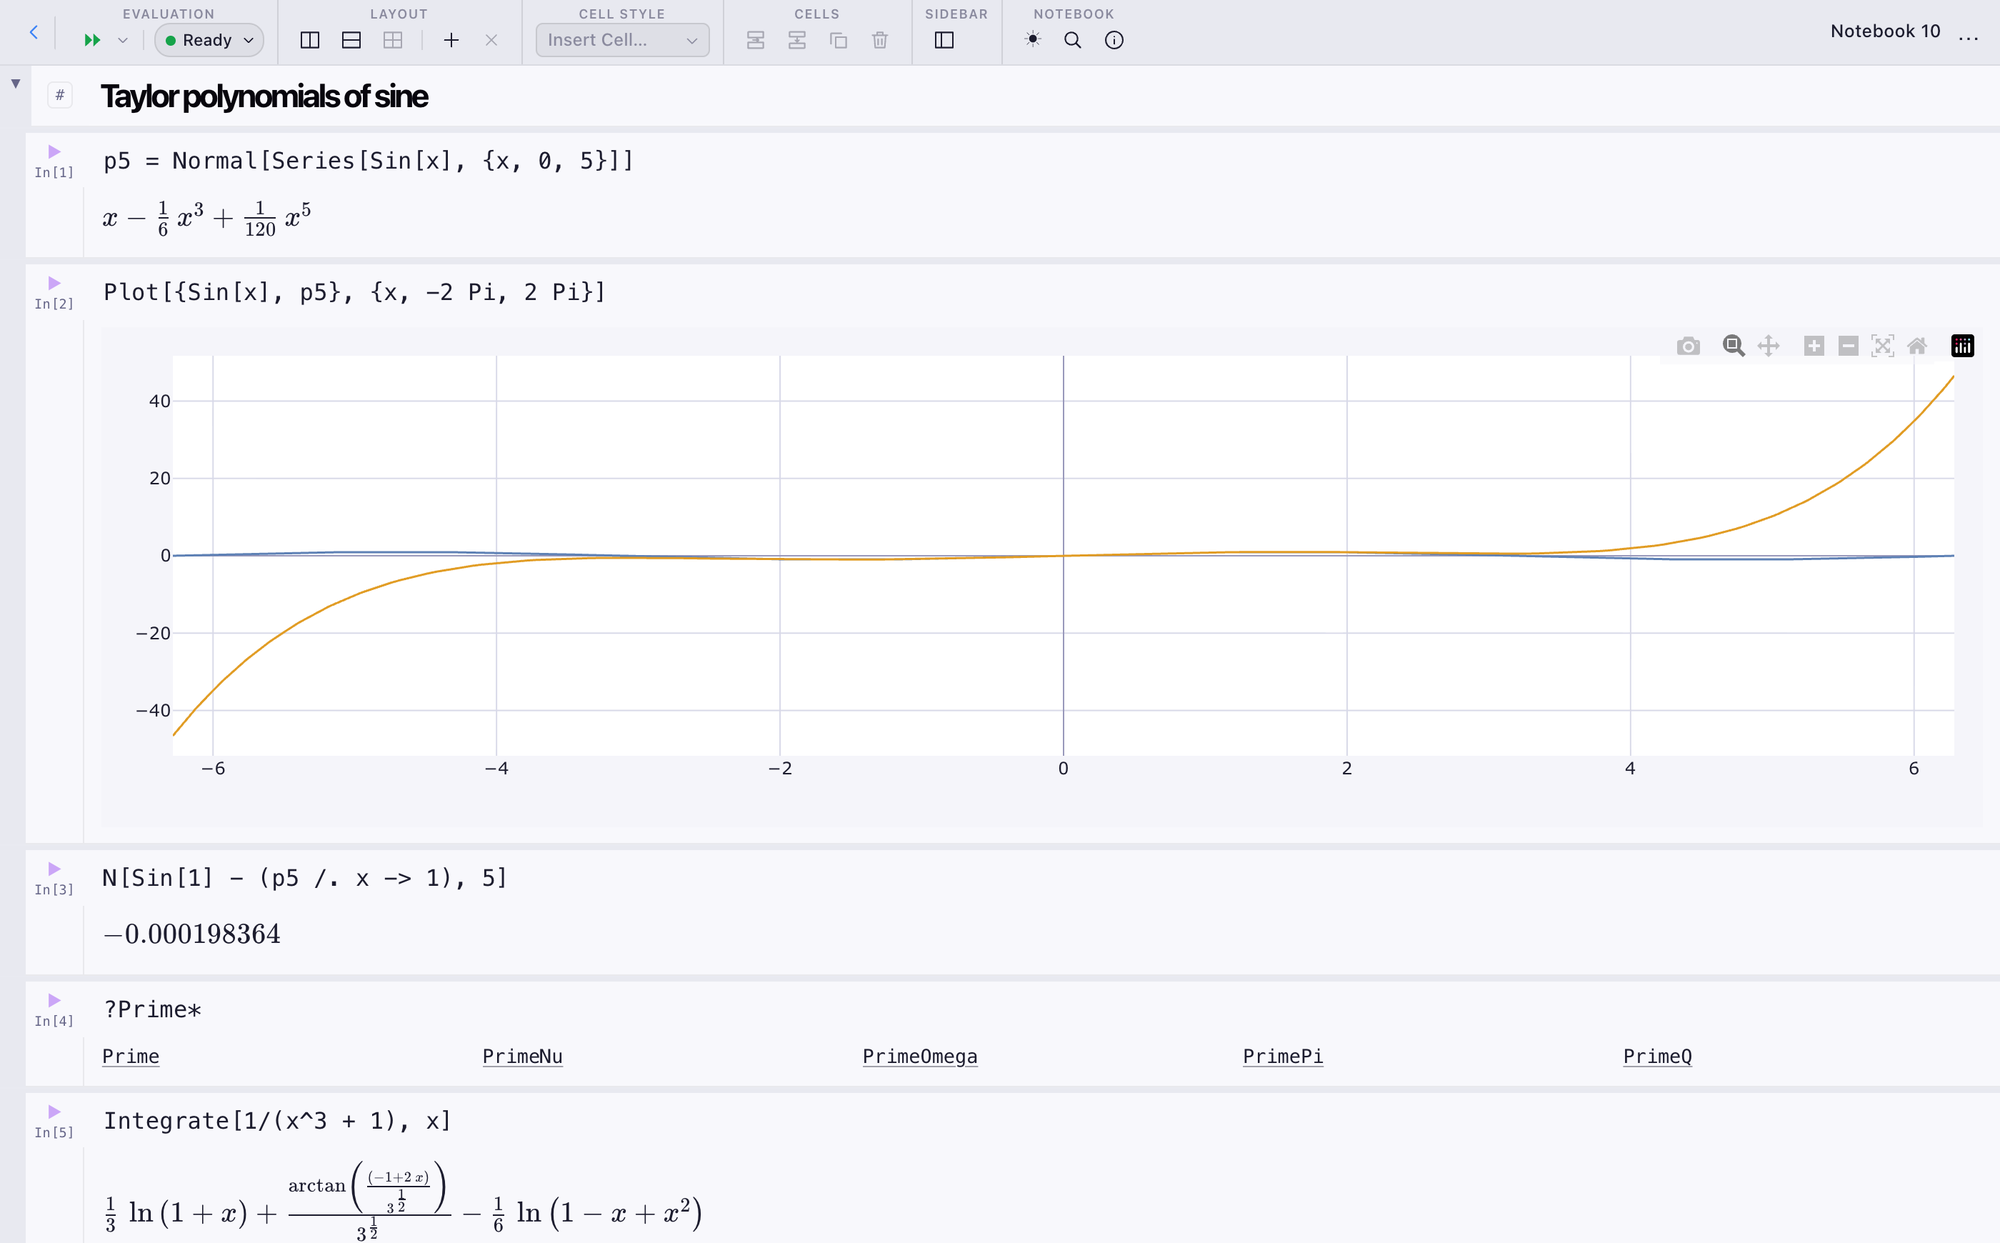
\includegraphics[width=\linewidth]{figures/notebook/explore.png}
  \caption{A Taylor polynomial, its plot against the sine, and its error at
  \(x = 1\).}
  \label{fig:nb-explore}
\end{figure}

\subsection*{Turn a 3D Volume}

Medical and microscopy data arrive as stacks of slices. Make a test volume and
look at it from several sides:

\begin{shell}
ball = Image3D[Table[If[(x-16)^2 + (y-16)^2 + (z-16)^2 < 144, 1., 0.], {z, 32}, {y, 32}, {x, 32}]]; GaussianFilter[ball, 2]
\end{shell}

\noindent The result is drawn as a box whose faces carry projections through
the blurred ball. Drag it to turn it, double-click to return to the standard
view, and compare with \B{Dilation}\mcode{[ball, 2]} in the next cell. The
three filters that looked identical under the old boundary rendering now
look different (\S\ref{ssec:nb-volumes}).

\subsection*{Resize an Image Inline}

A small image is magnified automatically, but you decide how big a picture
should be in a report. Click the image to select it, drag any corner, and the
note underneath reports the width you chose (Figure~\ref{fig:nb-image}).
Because every pixel is drawn as a sharp square, enlarging a small result,
say an \(8\times8\) \B{Binarize} mask, lets you read individual pixels.
Double-click to undo the resize.

\subsection*{Read the Documentation Without Leaving Your Cell}

You are halfway through an expression and cannot remember the arguments of
\B{PrimePi}. Put the caret in the name and press \texttt{F1}. The reference
page opens in a pane on the right, with its examples as live cells, and the
caret stays where it was (Figure~\ref{fig:nb-docpane}). Press \texttt{F1} on
another name and the same pane shows the new page.

\subsection*{Find a Function by Name}

Type \mcode{?Image*} in a cell and evaluate it. The answer is a grid of every
symbol whose name starts with \mcode{Image}, and each name is a button that
opens its page. For the complete list, choose \emph{Browse all symbols} from
the documentation menu, which opens a notebook evaluating \mcode{?*}.

\subsection*{Compare Two Notebooks Side by Side}

To check a new derivation against an old one, open the first notebook in
focused mode and press \texttt{Cmd+\textbackslash}. The next notebook on the
canvas joins it as a second pane, and the \emph{Add a notebook} button
offers the others by name. With three or four panes, the grid button tiles
them two by two (Figure~\ref{fig:nb-grid}). Remember that the panes share one
kernel, so a definition made in one is visible in the others.

\subsection*{Insert a Template and Fill It In}

With the caret in an empty code cell, choose \emph{Integrate} from the Insert
palette. The cell now reads \mcode{Integrate[expr, x]} with \mcode{expr}
selected. Type the integrand, press Tab to move to \mcode{x}, and press
\texttt{Shift+Enter}. Every template was parsed by the kernel before it was
shipped, so the brackets are always balanced.

\subsection*{Watch What a Computation Costs}

The status bar reports the duration of every evaluation and the kernel's
memory after it. Evaluate a large \B{Table} and watch the memory figure rise;
evaluate \mcode{Clear} on the variable and see whether it falls. The session
figure on the right sums every evaluation since the kernel last restarted,
which gives a quick total for a whole notebook after \emph{Evaluate notebook}.

\section{Limitations}
\label{sec:nb-limits}
\index{notebook!limitations}

The notebook is young, and some limitations have been mentioned along the
way. Collected in one place:

\begin{itemize}
\item \B{Print} output and kernel warning messages do not appear in cells
  (\S\ref{ssec:nb-lost}).
\item A cell is one expression. Separate statements with semicolons, and keep
  a cell under about ten kilobytes.
\item Abort restarts the kernel and loses all definitions. There is no
  cooperative interrupt.
\item One kernel serves every notebook, so notebooks share definitions and
  wait for each other.
\item Outputs, pane layout, zoom and preferences are not saved. There is no
  export to PDF or HTML.
\item The stanza \texttt{.mathilda} format exists in the Rust layer but is not
  wired to the interface, and the Open dialog cannot read it.
\item The Cell menu's \emph{Convert to} items do not retype the cell, and the
  properties panel and find bar open out of sight, in the build examined here.
\item The editor has no Mathilda syntax highlighting, bracket matching, or
  completion of symbol names.
\item Existing plots keep their colours when the theme changes.
\item Only macOS has been exercised; the Linux and Windows bundles are
  configured but untested. The iOS and Android builds cannot show images,
  help messages or names grids, and cannot restart or abort.
\end{itemize}

\subsection*{Where this connects}

The notebook is a client of the pipe mode introduced with the REPL in
\S\ref{sec:scripts}, and the kernel behind it is the one whose evaluator,
symbol table and printer are described in Chapter~\ref{ch:internals}. The
typeset output is the kernel's own \LaTeX{} form, the plots are the
\mcode{Graphics} objects of Chapter~\ref{ch:graphics} translated for Plotly,
and the images and volumes are those of Chapter~\ref{ch:images}, where the
filters used in this chapter's examples are explained. The reference pages
that the notebook opens beside your work are the same pages the website
publishes, verified against the binary in the same way this book's
transcripts are. If you want to change the notebook itself, the front end
lives in \texttt{frontend/}, and Chapter~\ref{ch:contributing} explains how
changes to Mathilda are reviewed and tested.
